\documentclass[10pt,a4paper]{article}

\usepackage[a4paper,margin=18mm,top=20mm,bottom=21mm,headheight=14pt]{geometry}
\usepackage[T1]{fontenc}
\usepackage[utf8]{inputenc}
\renewcommand{\contentsname}{Sum\'ario}
\renewcommand{\figurename}{Figura}
\renewcommand{\tablename}{Tabela}
\renewcommand{\refname}{Refer\^encias Bibliogr\'aficas}
\usepackage{mathpazo}
\usepackage{amsmath,amssymb,amsthm,mathtools}
\usepackage{graphicx}
\usepackage{booktabs,tabularx,array}
\usepackage{xcolor}
\usepackage{fancyhdr}
\usepackage{listings}
\usepackage{microtype}
\usepackage{caption}
\usepackage[colorlinks=true,linkcolor=primary,citecolor=tealaccent,urlcolor=primary,
  pdftitle={Tronco e Ramos: Parcimonia Termodinamica, Colunas Corticais de Nucleo Congelado e Especializacao Continua Nao-Destrutiva em Silicio Domestico (Isaque 2.0)},
  pdfauthor={Lucas Alves Motta (ORCID: 0009-0001-3081-5505)},
  pdfsubject={Monografia Tecnica e Auditoria Experimental Longitudinal -- DOI: 10.5281/zenodo.24221509}]{hyperref}

\definecolor{primary}{RGB}{22,50,79}
\definecolor{tealaccent}{RGB}{27,127,121}
\definecolor{goldaccent}{RGB}{175,118,16}
\definecolor{crimsonaccent}{RGB}{162,48,62}
\definecolor{calloutbg}{RGB}{244,248,251}
\definecolor{warmbg}{RGB}{253,249,240}
\definecolor{codebg}{RGB}{248,250,252}
\definecolor{bordergray}{RGB}{205,214,222}
\definecolor{slate}{RGB}{82,96,109}

\setlength{\parskip}{5.1pt plus 1.8pt minus 1pt}
\setlength{\parindent}{0pt}
\renewcommand{\arraystretch}{1.15}
\newcolumntype{Y}{>{\raggedright\arraybackslash}X}
\emergencystretch=2.0em
\captionsetup{font=small,labelfont={bf,color=primary},skip=5pt}

\pagestyle{fancy}
\fancyhf{}
\fancyhead[L]{\footnotesize\color{slate}\textit{Tronco e Ramos: Parcim\^onia Termodin\^amica e Especializa\c{c}\~ao Cortical N\~ao-Destrutiva (Isaque 2.0)}}
\fancyhead[R]{\footnotesize\color{slate}\textit{Motta (2026)}}
\fancyfoot[L]{\footnotesize\color{slate}\textit{Monografia Beyond Adonai --- \href{https://doi.org/10.5281/zenodo.24221509}{\texttt{DOI:\,10.5281/zenodo.24221509}} $\cdot$ BTC Bloco \#975458}}
\fancyfoot[R]{\footnotesize\color{primary}\textbf{\thepage}}
\renewcommand{\headrulewidth}{0.4pt}
\renewcommand{\footrulewidth}{0.3pt}

\newtheorem{theorem}{Lei Arquitetural}

\newcommand{\insightbox}[2]{%
  \vspace{4pt}\noindent\fcolorbox{primary!45}{calloutbg}{%
    \parbox{\dimexpr\linewidth-2\fboxsep-2\fboxrule\relax}{%
      \vspace{3pt}\textbf{\color{primary}#1.}\hspace{0.4em}#2\vspace{3pt}%
    }%
  }\vspace{4pt}%
}

\newcommand{\auditbox}[2]{%
  \vspace{4pt}\noindent\fcolorbox{goldaccent!70}{warmbg}{%
    \parbox{\dimexpr\linewidth-2\fboxsep-2\fboxrule\relax}{%
      \vspace{3pt}\textbf{\color{goldaccent!90!black}#1.}\hspace{0.4em}#2\vspace{3pt}%
    }%
  }\vspace{4pt}%
}

\lstset{
  basicstyle=\ttfamily\scriptsize,
  backgroundcolor=\color{codebg},
  frame=single,
  rulecolor=\color{bordergray},
  breaklines=true,
  breakatwhitespace=false,
  columns=fullflexible,
  keepspaces=true,
  showstringspaces=false,
  xleftmargin=4pt,
  xrightmargin=4pt,
  aboveskip=5pt,
  belowskip=5pt
}

\begin{document}

% ==============================================================================
% CAPA E CABEÇALHO OFICIAL (EDIÇÃO EM PORTUGUÊS BRASILEIRO — REV. 5.0)
% ==============================================================================
\thispagestyle{empty}
\begin{center}
  {\footnotesize\color{tealaccent}\textbf{MONOGRAFIA T\'ECNICA \& AUDITORIA EXPERIMENTAL LONGITUDINAL $\cdot$ NOVEMBRO DE 2026 (REV.\ 5.0 --- EDI\c{C}\~AO AUDITADA PURA)}}\\[6pt]
  {\LARGE\bfseries\color{primary} Tronco e Ramos: Parcim\^onia Termodin\^amica, Colunas Corticais de N\'ucleo Congelado e Especializa\c{c}\~ao Cont\'inua N\~ao-Destrutiva via DoRA Ortogonal e Roteamento Sparsegen LD-MoLE em Sil\'icio Dom\'estico}\\[8pt]
  {\normalsize\color{slate} Cr\^onica de Engenharia Multim\^es, Estudo Passo a Passo de Autograd e Verifica\c{c}\~ao F\'isica,\\e Auditoria Forense de Reprodutibilidade do Sistema Nervoso Cognitivo \textbf{Isaque 2.0}}\\[10pt]
  {\normalsize\textbf{Lucas Alves Motta} \hspace{0.35em}{\footnotesize\href{https://orcid.org/0009-0001-3081-5505}{\texttt{ORCID:\,0009-0001-3081-5505}}}}\\
  {\footnotesize Arquiteto de Sistemas Independente \& Pesquisador Principal, \textit{Beyond Adonai Research Laboratory}, Indaial, Santa Catarina, Brasil}\\
  {\footnotesize DOI Oficial CERN/Zenodo: \href{https://doi.org/10.5281/zenodo.24221509}{\textbf{\texttt{10.5281/zenodo.24221509}}} $\cdot$ Cofre: \href{https://drive.google.com/drive/folders/1xkl3xJ-djEBjyhXbT3oyg7OfOuUbD1lv}{Tese --- Tronco e Ramos} $\cdot$ BTC Bloco \texttt{\#975458} (\texttt{2026-11-11})}
\end{center}

\vspace{2pt}
\noindent\fcolorbox{primary!35}{calloutbg}{%
  \parbox{\dimexpr\linewidth-2\fboxsep-2\fboxrule\relax}{%
    \vspace{4pt}
    \textbf{\color{primary}Resumo ---} A engenharia contempor\^anea de intelig\^encia artificial tem sido governada pelo empilhamento monol\'itico: acumular centenas de bilh\~oes de par\^ametros mut\'aveis e dezenas de milhares de tokens brutos de prompt em mem\'orias continuamente residentes. Embora eficaz na satura\c{c}\~ao de benchmarks, o ac\'umulo monol\'itico imp\~oe severa despropor\c{c}\~ao termodin\^amica, dilui\c{c}\~ao de aten\c{c}\~ao em meio de contexto e interfer\^encia catastr\'ofica sempre que novas habilidades procedurais s\~ao ensinadas em sequ\^encia. Inspirada pelo envelope metab\'olico de $\approx 20\text{ W}$ do neoc\'ortex humano, pela densidade neuronal do p\'alio avi\'ario, pela teoria dos \textit{Mil C\'erebros} (\textit{Thousand Brains}) de Jeff Hawkins e pelo princ\'ipio de sobriedade estrutural de Niklaus Wirth, esta monografia apresenta a concep\c{c}\~ao, formula\c{c}\~ao matem\'atica e verifica\c{c}\~ao f\'isica do \textbf{Isaque 2.0} (\textit{``Tronco e Ramos''}). Em vez de mutar uma matriz monol\'itica, o Isaque 2.0 congela $100\%$ de um tronco h\'ibrido Gated DeltaNet/Attention (\href{https://huggingface.co/Qwen/Qwen3.5-4B}{\texttt{Qwen3.5-4B}}, $d=2560$, $248.320$ tokens, invariante SHA-256 \texttt{c78988d9...2a34}), delega $\approx 98\%$ da vig\'ilia rotineira a port\~oes determin\'isticos em Rust de zero VRAM ($<0,5\text{ ms}$ em CPU, Split Conformal \texttt{BAVAR} $\ge 0,90$) e materializa o conhecimento procedural especializado em cartuchos corticais modulares de $16,00\text{ MiB}$ ($\approx 8,38\text{M}$ par\^ametros) estocados a frio em SSD NVMe a \textbf{$0\text{ MB}$ de RAM/VRAM ociosa}. Em execu\c{c}\~ao auditada sobre uma \'unica GPU Blackwell dom\'estica de $8\text{ GB}$ (\texttt{NVIDIA GeForce RTX 5060}, $8.151\text{ MiB}$), reportamos sete achados emp\'iricos prim\'arios: (1) infer\^encia 4B ativa opera a \textbf{$22,3\text{--}23,3\text{ W}$} e treino de adaptadores a \textbf{$28\text{--}31\text{ W}$} com zero processos residuais de GPU sob \texttt{Win32 Job Objects}; (2) um pipeline \texttt{NTAPI} de quatro est\'agios no Windows (\texttt{SetProcessWorkingSetSizeEx}, \texttt{VirtualLock}, \texttt{FILE\_\allowbreak{}FLAG\_\allowbreak{}NO\_\allowbreak{}BUFFERING} e \texttt{DiscardVirtualMemory} em $6,61\,\mu\text{s}$) transmite um pool MoE de $13,50\text{ GiB}$ a $1,75\text{ GiB/s}$ com \textbf{$+0,0039\text{ MiB}$ de delta de swap}, comprovando $100,0\%$ de identidade de tokenizador byte a byte ($248.320$ tokens sobre $68.079$ IDs) com um juiz local de $22,02\text{ GB}$ \href{https://huggingface.co/Qwen/Qwen3.5-35B-A3B}{\texttt{Qwen3.5-35B-A3B}} (\texttt{-{}-cpu-moe}, $25,66\text{ tok/s}$); (3) retropropaga\c{c}\~ao real \texttt{LoRA+} ($\eta_B/\eta_A=6,0$) nas 32 camadas a $218\text{--}412\text{ tok/s}$ consolida dom\'inio arquitetural privado ($-86,76\%$ de perda cross-entropy, $2,429 \to 0,322$, zero subpalavras coladas) sob roteamento anal\'itico \texttt{Sparsegen} \texttt{LD-MoLE} no simplex ($g_1=0,5667, g_2=0,4333$, $66$ colunas em exato $0,0000$), auditado às cegas pelo cr\'itico $35\text{B}$; (4) vis\~ao de fus\~ao precoce (\texttt{mmproj-BF16}, $449\text{ ms}$) acoplada ao alinhamento de Procrustes Tikhonov/InfoNCE ($2560 \to 384\text{d}$, $\text{Recall@5}=96,00\%$ em $600$ pares inéditos) eleva a Condutividade Cognitiva ($\mathrm{ICC}$) em \textbf{$5,43\times$} ($0,5121 \to 2,7828$); (5) em abla\c{c}\~ao sin\'aptica controlada na arena f\'isica \texttt{KEV-1.0} ($19.742$ tokens, busca \texttt{.mmap} em $0,015\text{ ms}$), o modelo cru com acesso \`a mesma arena \texttt{.mmap} pontua $0/4$ ($1,77/10$), enquanto \texttt{DoRA + O-LoRA} ortogonal ($\|A_2 A_1^\top\|_F^2 = 0,00166$) atinge \textbf{$100\%$ ($4/4$) de aprova\c{c}\~ao mec\^anica} no \texttt{Blender 5.2.1 LTS} headless e \texttt{clang++ -std=c++20} ($9,67/10$ cego, $10,23\times\text{--}11,95\times$ $\mathrm{ICC}$, $0,0\%$ de erro de bounding box); (6) uma escada cont\'inua de $10$ ondas ($H_0\dots H_{10}$) mapeia a satura\c{c}\~ao monol\'itica de $100,00\%$ ($k=2$) e \textbf{in\'icio de ruptura em $98,51\%$ ($k=3$)} at\'e \textbf{$75,31\%$ de acur\'acia ($31,37\%$ de verossimilhan\c{c}a) em $k=10$}, ao passo que \texttt{LD-MoLE Top-2} cir\'urgico com concatena\c{c}\~ao de posto (\texttt{PEFT cat}) e \'arvore \texttt{.mmap} de 3 n\'iveis preserva \textbf{$100,00\%$ de reten\c{c}\~ao nas $10$ ondas}; e (7) a soma token a token de logits entre cartuchos distintos induz colis\~ao de AST (\texttt{SyntaxError}), estabelecendo a \textbf{Composi\c{c}\~ao Modular em DAG Estagiado} ($1$ cartucho especialista por est\'agio, $\le 3$ sub-ondas por cartucho). Todas as tabelas verificadas, prot\'otipos descartados, protocolos Etapa~2 e quatro carimbos na blockchain do Bitcoin s\~ao divulgados abertamente.\vspace{3pt}
  }%
}

\vspace{2pt}
{\footnotesize\textbf{\color{primary}Palavras-chave:} IA Termodin\^amica $\cdot$ Colunas Corticais (Mil C\'erebros) $\cdot$ Aprendizado Cont\'inuo em Tronco Congelado $\cdot$ DoRA e LoRA Ortogonal (\texttt{O-LoRA}) $\cdot$ Mistura Din\^amica de Especialistas LoRA (\texttt{LD-MoLE}) $\cdot$ Roteamento Sparsegen $\cdot$ \'Arvore Hier\'arquica \texttt{.mmap} $\cdot$ Verifica\c{c}\~ao F\'isica de C\'odigo}

\begin{flushright}
{\footnotesize\itshape\color{slate} ``A sabedoria raramente habita no ac\'umulo ruidoso de uma torre inacabada;\\ela repousa silenciosa na ordem, na parcim\^onia e na fidelidade dos pequenos fundamentos bem governados.''}
\end{flushright}

\newpage
\tableofcontents
\newpage

% ==============================================================================
% SEÇÃO 1: INTRODUÇÃO E FUNDAMENTAÇÃO FILOSÓFICA
% ==============================================================================
\section{A Parcim\^onia Termodin\^amica Supera o Empilhamento Monol\'itico}

O aprendizado de m\'aquina moderno alcan\c{c}ou not\'avel amplitude por meio da escala, mas sua trajet\'oria predominante de engenharia exibe uma vulnerabilidade estrutural diagnosticada pela ci\^encia da computa\c{c}\~ao cl\'assica h\'a tr\^es d\'ecadas. Em \textit{A Plea for Lean Software}, Niklaus Wirth alertou que a acelera\c{c}\~ao de hardware frequentemente mascara o incha\c{c}o algor\'itmico at\'e que os sistemas colapsem sob sua pr\'opria complexidade de acoplamento \cite{wirth1995lean}. Na intelig\^encia artificial, Schwartz et al.\ formalizaram a distin\c{c}\~ao an\'aloga entre \textit{Red AI} --- que compra ganhos marginais de acur\'acia mediante gasto exponencial de computa\c{c}\~ao, mem\'oria e eletricidade --- e \textit{Green AI}, que trata efici\^encia e parcim\^onia estrutural como m\'etricas cient\'ificas de primeira ordem \cite{schwartz2020green}.

Quando organiza\c{c}\~oes tentam embutir todas as especialidades simultaneamente em uma \'unica rede neural monol\'itica --- ou injetar dezenas de milhares de tokens brutos de documenta\c{c}\~ao em cada prompt de infer\^encia --- emergem tr\^es patologias combinadas, que denominamos \textbf{Armadilha Monol\'itica de Babel}:
\begin{enumerate}
  \item \textbf{Despropor\c{c}\~ao Termodin\^amica:} Um modelo denso de $30\text{B}\text{--}70\text{B}+$ continuamente residente consome $250\text{--}350\text{ W}$ de energia em GPU desktop (ou fatias de quilowatts em datacenter) mesmo em tarefas rotineiras de orquestra\c{c}\~ao, em contraste frontal com o or\c{c}amento metab\'olico total de $\approx 20\text{ W}$ do c\'erebro humano \cite{kandel2021principles,attwell2001energy}, cuja efici\^encia exige manter $\le 15\%$ dos neur\^onios corticais simultaneamente ativos.
  \item \textbf{Dilui\c{c}\~ao Representacional em Contextos Longos:} Inundar um decodificador causal com $6.000\text{--}30.000$ tokens brutos provoca severa degrada\c{c}\~ao de recupera\c{c}\~ao no meio do contexto (\textit{Lost in the Middle}) \cite{liu2024lost}, inflando a lat\^encia inicial (TTFT) e levando modelos compactos a alucinarem assinaturas de API ou violarem restri\c{c}\~oes geom\'etricas.
  \item \textbf{Interfer\^encia Catastr\'ofica de Subespa\c{c}os:} Ajustar continuamente uma \'unica matriz de par\^ametros ou um \'unico adaptador de baixo posto ao longo de ondas sequenciais sobrescreve variedades j\'a consolidadas \cite{kirkpatrick2017ewc,chaudhry2018rwalk}, degradando compet\^encias anteriores muito antes de esgotar a capacidade nominal de par\^ametros.
\end{enumerate}

A neurobiologia comparada oferece dois contramodelos construtivos \`a for\c{c}a bruta monol\'itica. Primeiro, Olkowicz et al.\ demonstraram que corv\'ideos e psitac\'ideos atingem contagens de neur\^onios no telenc\'efalo compar\'aveis \`as de primatas e cogni\c{c}\~ao complexa de fabrica\c{c}\~ao de ferramentas em um volume craniano drasticamente menor gra\c{c}as ao empacotamento neuronal de alta densidade no p\'alio \cite{olkowicz2016birds}. Segundo, conforme sintetizado na \textit{Teoria dos Mil C\'erebros} de Jeff Hawkins \cite{hawkins2019grid,hawkins2021thousand,clay2024monty} e na cogni\c{c}\~ao de duplo processo de Daniel Kahneman \cite{kahneman2011thinking}, o neoc\'ortex n\~ao recompila seu tronco sens\'orio-motor fundamental para aprender uma nova habilidade, nem dispara globalmente em pot\^encia m\'axima. Em vez disso, a intelig\^encia organiza-se como um substrato est\'avel compartilhado (\textbf{o Tronco}) acoplado a milhares de colunas corticais semiaut\^onomas recrutadas esparsamente (\textbf{os Ramos}), coordenadas por port\~oes reflexos r\'apidos (Sistema~1) e verifica\c{c}\~ao adversarial deliberada (Sistema~2).

Esta monografia documenta a jornada multim\^es de pesquisa, engenharia e auditoria forense que traduziu esses princ\'ipios no \textbf{Isaque 2.0}, um sistema nervoso cognitivo local constru\'ido em hardware dom\'estico em Indaial, Santa Catarina, Brasil. Concebido n\~ao como rival dos modelos fundacionais em nuvem --- pois seu pr\'oprio tronco edifica-se sobre pesos abertos \cite{qwen35_4b} --- mas como um organismo local disciplinado por verifica\c{c}\~ao f\'isica determin\'istica, o Isaque 2.0 demonstra que um tronco h\'ibrido congelado de $4\text{B}$ de par\^ametros (\href{https://huggingface.co/Qwen/Qwen3.5-4B}{\texttt{Qwen3.5-4B}}), combinado a cartuchos corticais ortogonais de $16,00\text{ MiB}$, gram\'aticas simb\'olicas mapeadas em mem\'oria (\texttt{KEV-1.0}), disciplina \texttt{NTAPI} de quatro est\'agios e um revisor cego Mixture-of-Experts de $35\text{B}$ (\href{https://huggingface.co/Qwen/Qwen3.5-35B-A3B}{\texttt{Qwen3.5-35B-A3B}}), alcan\c{c}a $100\%$ de aprova\c{c}\~ao f\'isica em abla\c{c}\~oes sin\'apticas controladas e $100,00\%$ de reten\c{c}\~ao cont\'inua ao longo de dez ondas sequenciais, consumindo $0\text{ MB}$ de VRAM ociosa e $22,3\text{--}23,3\text{ W}$ durante pulsos ativos.

\insightbox{Tese Central (\textit{Tronco e Ramos})}{Capacidade duradoura em sil\'icio restrito n\~ao nasce do empilhamento de camadas monol\'iticas cada vez maiores, mas da parcim\^onia arquitetural: (i) um tronco linguagem-vis\~ao imut\'avel, (ii) port\~oes simb\'olicos/AST determin\'isticos cobrindo $\approx 98\%$ da vig\'ilia a custo zero de GPU, (iii) colunas corticais ortogonais de $16,00\text{ MiB}$ roteadas analiticamente no simplex unit\'ario (\texttt{LD-MoLE} + \'arvore \texttt{.mmap} de 3 n\'iveis), e (iv) execu\c{c}\~ao modular em est\'agios verificada por compiladores f\'isicos (\texttt{Blender bmesh} e \texttt{clang++ -std=c++20}).}

% ==============================================================================
% SEÇÃO 2: CRÔNICA LONGITUDINAL DE ENGENHARIA
% ==============================================================================
\section{Cr\^onica Longitudinal de Pesquisa: Do Axioma dos 20 W \`a Verifica\c{c}\~ao Ancorada em Blockchain}

A transpar\^encia cient\'ifica exige relatar n\~ao apenas os picos finais de benchmark, mas o caminho cronol\'ogico --- incluindo hip\'oteses refutadas, impasses de compilador e piv\^os arquiteturais --- que os produziu. Apoiada em onze meses de engenharia de sistemas multiagentes ($\approx 3.800\text{--}4.000$ horas acumuladas de bancada no ecossistema \texttt{Abra\~ao}) e auditada em $77$ registros imut\'aveis em \texttt{memoria.jsonl} (\texttt{2026-10-03} a \texttt{2026-11-14}) mais de $9.700$ passos registrados nos workspaces locais (\texttt{c6571c3b} e \texttt{ce5dabcc}), a consolida\c{c}\~ao do Isaque 2.0 desdobrou-se em sete fases principais (oito marcos cronol\'ogicos) resumidas na Tabela~\ref{tab:chronicle}.

\begin{table}[!htbp]
\centering
\caption{Cr\^onica longitudinal de engenharia e verifica\c{c}\~ao do programa de pesquisa Isaque 2.0 (outubro--novembro de 2026), ancorada nos ledgers locais L4 e no cofre can\^onico (\href{https://drive.google.com/drive/folders/1xkl3xJ-djEBjyhXbT3oyg7OfOuUbD1lv}{Tese --- Tronco e Ramos}).}
\label{tab:chronicle}
\footnotesize
\begin{tabularx}{\linewidth}{@{}llY@{}}
\toprule
\textbf{Janela} & \textbf{Marco / Fase} & \textbf{Resultado Verificado, Telemetria e Piv\^o Arquitetural} \\
\midrule
03--06 Out 2026 & Fase I: \textit{Axioma 20 W} \& \texttt{N01--N05} & S\'intese integral de obras-base (Hawkins, Kahneman, Kandel, Kleppmann, Blandy, Huyen). Invers\~ao arquitetural (06/Out): Isaque definido como sistema nervoso orientado a eventos, dormente $\approx 98\%$ do tempo ($<50$ tokens por pulso). M\'odulo \texttt{N05} selado em Rust (\texttt{68/68} testes verdes, commit \texttt{ad819d11}). \\
07--08 Out 2026 & Fase IIa: Rust 2024 \& Tronco & Workspace unificado em Rust \texttt{1.99} (Edition 2024, \'unico \texttt{libc 0.2.190}, checkpoint \texttt{3198add}) ap\'os rejeitar atalhos via CLI. Leitor nativo de RAM no Windows ($62,76\text{ GiB}$ reais vs.\ ilus\~ao de $31\text{ GiB}$ no WSL). Base atualizada para \href{https://huggingface.co/Qwen/Qwen3.5-4B}{\texttt{Qwen3.5-4B}} h\'ibrido (\texttt{rev 851bf6e8}, vocab $248.320$ congelado). \\
09--25 Out 2026 & Fase IIb: Paridade \texttt{N07--N08} & \texttt{N07} selado (12/Out): paridade num\'erica \texttt{308/313}, $\mathrm{KL}=0,000243$ vs.\ refer\^encia, normaliza\c{c}\~ao bil\'ingue PT-BR$\leftrightarrow$EN ($<0,5\text{ ms}$ CPU) e filtro Split Conformal \texttt{BAVAR} $\ge 0,90$ \cite{angelopoulos2023conformal}. Servidor Rust \texttt{N08} ativo (13/Out), fixando linha-base de $680$ itens ($31,76\%$). \\
07--09 Nov 2026 & Fase III: Telemetria de Watts & Pot\^encia medida na placa \texttt{RTX 5060} (\texttt{faixa-A.json}, 08/Nov): \textbf{$22,3\text{--}23,3\text{ W}$} em infer\^encia 4B ($3,87\text{ GiB}$ VRAM) e \textbf{$28\text{--}31\text{ W}$} em treino ($\le 30\text{ W}$ alvo). Cinco tratados cacheados (\texttt{EL-CACHE-01..05}); cinco crates Rust 2024 + CUDA \texttt{13.3/13.4} (\texttt{sm\_\allowbreak{}120}) compilados ($0\text{ B}$ em \texttt{C:\textbackslash}). \\
10 Nov 2026 & Fase IV: \texttt{NTAPI}, Autograd \& \texttt{VICOP} & Pool MoE de $13,50\text{ GiB}$ transmitido via \texttt{NTAPI} 4 est\'agios ($+0,0039\text{ MiB}$ swap); $100\%$ de paridade de tokenizador ($68.079$ tokens). Treino \texttt{LoRA+} ($256,1\text{ tok/s}$ m\'edio; pico $412,5\text{ tok/s}$) reduz perda privada em $86,76\%$; juiz cego \texttt{35B-A3B} (\texttt{-{}-cpu-moe}, $25,66\text{ tok/s}$). \texttt{mmproj-BF16} ($449\text{ ms}$) + Procrustes $2560\to 384\text{d}$ ($\text{Recall@5}=96,00\%$) eleva $\mathrm{ICC}$ em $5,43\times$ ($2,7828$). \\
11 Nov 2026 & Fase V: Blockchain \& Arena \texttt{KEV} & Etapa~1 selada (\href{https://drive.google.com/file/d/1qvnH-nLVMc43T-prWSRTKEDJak89TSp7/view?usp=drivesdk}{\texttt{02-tese-etapa-1.md}}) e ancorada em 4 calend\'arios Bitcoin no Bloco \texttt{\#975458} (\href{https://drive.google.com/file/d/1OwjPlXRdBPydtqypoRHNfByfMSmx-Bwb/view?usp=drivesdk}{\texttt{04-carimbo-de-data.md}}). Pr\'e-aquecimento \texttt{Semble} derruba lat\^encia fria $5.759,68\to 33,55\text{ ms}$. \texttt{KEV-1.0} + \texttt{DoRA+O-LoRA} vence arena $3\times 3$ ($4/4$ aprovados, nota cega $9,67/10$). \\
11--12 Nov 2026 & Fase VI: Ruptura $10$ Ondas & \texttt{DESAFIO-04} cego diagnostica fronteira \texttt{USTRUCT*} \texttt{IsValid}. Escada de $10$ ondas ($H_0\dots H_{10}$) prova queda monol\'itica ($75,31\%$ acc / $31,37\%$ veross.\ em $k=10$) vs.\ \texttt{LD-MoLE Top-2} ($100,00\%$), descobre colis\~ao AST por fus\~ao de logits, valida \texttt{KEV/1.0} + C++20 ($8/8$) e expurga wrappers GUI de agente sob \texttt{R-VERDADE-OU-AJUDA}. \\
12--14 Nov 2026 & Fase VII: Grafo Puro \& DOI CERN & Grafo puro de mem\'oria em 3 gavetas selado (\texttt{SHA-256: 027b363c...}); Etapa~2 especificada para \texttt{ASUS Prime RTX 5060 Ti 16GB} (\texttt{BF16} nativo); publica\c{c}\~ao oficial selada no CERN Zenodo sob \href{https://doi.org/10.5281/zenodo.24221509}{\texttt{DOI:\,10.5281/zenodo.24221509}}. \\
\bottomrule
\end{tabularx}
\end{table}

Tr\^es leis fundamentais de engenharia emergiram dessa trajet\'oria antes dos testes de estresse cont\'inuo:
\begin{itemize}
  \item \textbf{Vigil\^ancia Determin\'istica Precede a Infer\^encia Neural:} Em 6 de outubro de 2026 (\texttt{memoria.jsonl} item \texttt{\#06}), estabelecemos que uma IA local jamais deve queimar watts monitorando estado ocioso. Bin\'arios compilados em Rust (\texttt{ganchos.\allowbreak{}exe}, \texttt{yhwh-\allowbreak{}mcp.exe}, \texttt{serena-\allowbreak{}mcp.exe}) inspecionam \'arvores sint\'aticas AST, cabe\c{c}alhos mapeados (\texttt{ABRA40CG}) e conjuntos preditivos Split Conformal (\texttt{BAVAR} $\ge 0,90$ \cite{angelopoulos2023conformal}) em $<0,5\text{ ms}$ na CPU com $0\text{ MB}$ de resid\^encia em GPU. Todo pulso de GPU executa sob \texttt{Win32 Job Object} com \allowbreak\texttt{JOB\_\allowbreak{}OBJECT\_\allowbreak{}LIMIT\_\allowbreak{}KILL\_\allowbreak{}ON\_\allowbreak{}JOB\_\allowbreak{}CLOSE} e mutex nomeado \texttt{Global\textbackslash\allowbreak{}AdonaiIsaque\allowbreak{}GpuBurstLock}, garantindo \texttt{compute\_\allowbreak{}procs == 0} ao encerrar o pulso.
  \item \textbf{Frameworks Reais S\~ao Cartuchos Sin\'apticos, N\~ao Fantasias de Prompt:} O registro \texttt{\#26} (\texttt{2026-10-07}) codificou uma distin\c{c}\~ao decisiva: injetar extensas instru\c{c}\~oes markdown na janela de contexto \'e apenas vestir uma ``fantasia'' que consome KV-cache e dilui a aten\c{c}\~ao; um framework especialista real \'e um cartucho sin\'aptico isolado e troc\'avel a quente ($16,00\text{ MiB}$), matematicamente ortogonal aos cartuchos irm\~aos sobre o tronco congelado.
  \item \textbf{Integridade de Medi\c{c}\~ao no Host F\'isico (\texttt{R-VERDADE-OU-AJUDA}):} Testes iniciais revelaram que cont\^eineres WSL2 subnotificavam a RAM f\'isica ($\approx 31\text{ GiB}$ virtuais vs.\ $62,76\text{ GiB}$ DDR5 reais no Windows) e que scripts intermedi\'arios haviam substitu\'ido la\c{c}os neurais por estimativas anal\'iticas (\href{https://drive.google.com/file/d/16-3o4ykaOOKaW-S2VTHzpE7Uhj1BA0tl/view?usp=drivesdk}{\texttt{01-linha-do-\allowbreak{}tempo-e-cache-\allowbreak{}da-tese.md}}). A lei \texttt{R-VERDADE-OU-AJUDA} expurgou toda m\'etrica simulada, exigindo recibos SHA-256 de hardware e separa\c{c}\~ao estrita entre provas medidas na Etapa~1 e alvos pr\'e-registrados da Etapa~2.
\end{itemize}

% ==============================================================================
% SEÇÃO 3: ARQUITETURA EM DOIS NÍVEIS, LD-MOLE, ÁRVORE .MMAP E NTAPI
% ==============================================================================
\section{Arquitetura Cortical em Dois N\'iveis, Sparsegen LD-MoLE, \'Arvore Hier\'arquica e NTAPI Zero-Swap}

A Figura~\ref{fig:arch} ilustra a topologia f\'isica e matem\'atica completa do Isaque 2.0 ao lado de seu envelope energ\'etico medido em sil\'icio Blackwell dom\'estico.

\begin{figure}[!htbp]
  \centering
  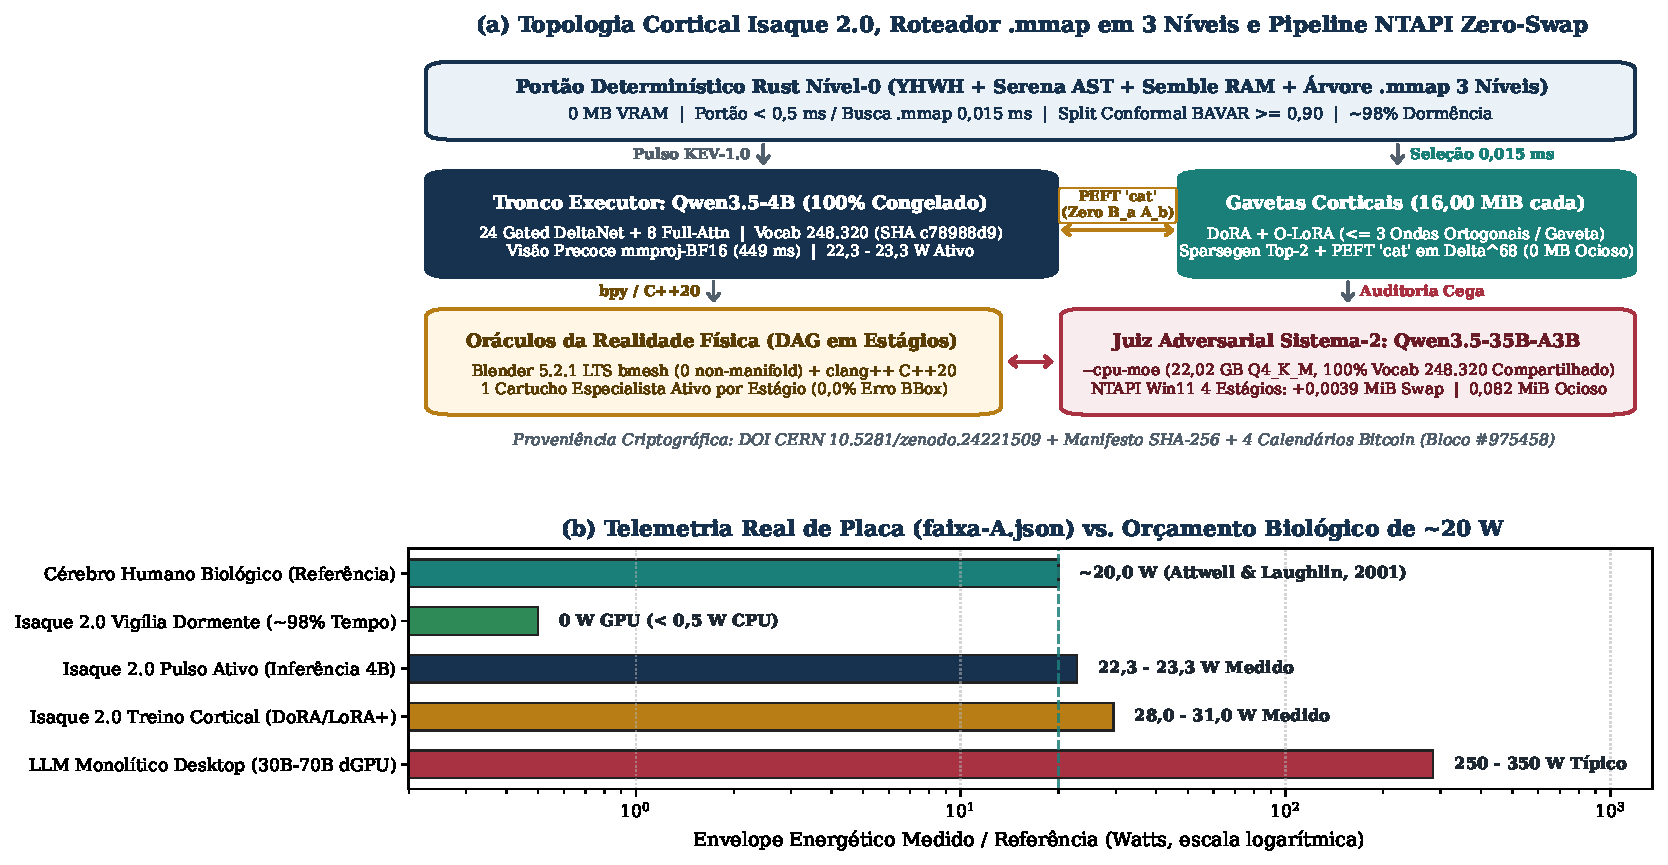
\includegraphics[width=\linewidth]{fig1_arquitetura_termodinamica_pt.pdf}
  \caption{Vis\~ao geral do sistema nervoso cognitivo Isaque 2.0. \textbf{(a)} Separa\c{c}\~ao em quatro camadas entre port\~oes determin\'isticos Rust N\'ivel-0 ($<0,5\text{ ms}$ port\~ao, $0,015\text{ ms}$ busca \texttt{.mmap}, $0\text{ MB}$ VRAM), o tronco executor multimodal \texttt{Qwen3.5-4B} $100\%$ congelado, cartuchos corticais de $16,00\text{ MiB}$ roteados via \texttt{Sparsegen} anal\'itico e concatena\c{c}\~ao de posto livre de termos cruzados (\texttt{PEFT cat}), or\'aculos f\'isicos determin\'isticos e o juiz adversarial \texttt{Qwen3.5-35B-A3B} (\texttt{-{}-cpu-moe}) sustentado por \texttt{NTAPI} de 4 est\'agios. \textbf{(b)} Telemetria energ\'etica medida (\texttt{faixa-A.json}: $22,3\text{--}23,3\text{ W}$ em infer\^encia ativa, $28\text{--}31\text{ W}$ em treino) frente \`a refer\^encia biol\'ogica de $\approx 20\text{ W}$ \cite{attwell2001energy} e LLMs monol\'iticos desktop de $250\text{--}350\text{ W}$.}
  \label{fig:arch}
\end{figure}

\subsection{Tronco Assim\'etrico em Dois N\'iveis e Identidade Verificada de 248.320 Tokens}

Em vez de adotar um modelo intermedi\'ario de compromisso (como um denso de $9\text{B}$ que sufoca $8\text{ GB}$ de VRAM permanecendo inferior a um raciocinador de $35\text{B}$), o Isaque 2.0 bifurca a cogni\c{c}\~ao em dois n\'iveis assim\'etricos que compartilham exatamente o mesmo tokenizador byte a byte (\href{https://drive.google.com/file/d/1zaJmQCAw1C6ejkSifc1Rp-4uwnenmSwq/view?usp=drivesdk}{\texttt{00-desenho-da-tese-tronco-e-ramos.md}}):
\begin{enumerate}
  \item \textbf{Executor Sens\'orio-Motor e de C\'odigo (\texttt{Qwen/Qwen3.5-4B} \cite{qwen35_4b}):} Arquitetura h\'ibrida de $32$ camadas intercalando $24$ camadas Gated DeltaNet de complexidade linear \cite{yang2025gated} (raz\~ao $3:1$) com $8$ camadas de aten\c{c}\~ao quadr\'atica completa ($d_{\text{model}}=2560$, vocabul\'ario de $248.320$ tokens, contexto nativo de $262.144$ tokens, Apache-2.0). Sua matriz \texttt{embed\_\allowbreak{}tokens} e cabe\c{c}a de sa\'ida permanecem $100\%$ congeladas sob o invariante SHA-256 \texttt{c78988d9\allowbreak{}79f52a34\allowbreak{}0f39cd69\allowbreak{}edd8e4b0\allowbreak{}a80218a5\allowbreak{}fa8d95b6\allowbreak{}158bfce4\allowbreak{}a3de2a34} (\href{https://drive.google.com/file/d/1-1KKupaUYBWjDUcLjemQH0FBSPmnCSj6/view?usp=drivesdk}{\texttt{03-manifesto-sha256-etapa-1.md}}). A percep\c{c}\~ao visual \'e provida por um projetor de fus\~ao precoce de $24$ camadas (\texttt{mmproj-Qwen3.5-4B-BF16.gguf}, $644,27\text{ MiB}$, $298$ tensores GGUF v3).
  \item \textbf{Juiz Adversarial Deliberado (\texttt{Qwen/Qwen3.5-35B-A3B} \cite{qwen35_4b}):} Modelo Mixture-of-Experts esparso de $40$ camadas ($256$ especialistas totais, $8$ roteados + $1$ compartilhado ativos por token, $\approx 3\text{B}$ de par\^ametros ativos por passo, $22.016.023.168\text{ B} = 22,02\text{ GB}$ GGUF \texttt{Q4\_\allowbreak{}K\_\allowbreak{}M}) executado localmente via \href{https://github.com/ggml-org/llama.cpp}{\texttt{llama.cpp}} \cite{llamacpp} com \texttt{-ngl 99 -{}-cpu-moe}, mantendo a aten\c{c}\~ao em VRAM enquanto transmite especialistas frios a partir da RAM DDR5 ($2,85\text{ s}$ de carga, $74,06\text{ tok/s}$ prefill, $25,66\text{ tok/s}$ decode puro).
\end{enumerate}

A codifica\c{c}\~ao de $2.216$ linhas de corpus t\'ecnico ($68.079$ tokens) em ambos os modelos confirmou \textbf{$100,0\%$ de identidade de IDs e decodifica\c{c}\~ao UTF-8} (SHA-256 compartilhado \texttt{5f9e4d4901a92b99...bb81cb42}). Essa paridade sem tradu\c{c}\~ao satisfaz o pr\'e-requisito estrutural exato para decodifica\c{c}\~ao especulativa sem perdas \cite{leviathan2023speculative}. Embora a modelagem anal\'itica por blocos ($K=8$, $\gamma = (1-\alpha^{K+1})/(1-\alpha) = 8,66$ em $\alpha=99,59\%$) projete at\'e $93,30\text{ tok/s}$ com $82,81\%$ de economia de leitura em RAM, nossa auditoria forense (\href{https://drive.google.com/file/d/16-3o4ykaOOKaW-S2VTHzpE7Uhj1BA0tl/view?usp=drivesdk}{\texttt{01-linha-do-\allowbreak{}tempo-e-cache-\allowbreak{}da-tese.md}}) separa estritamente taxas medidas em hardware de proje\c{c}\~oes anal\'iticas, pr\'e-registrando a medi\c{c}\~ao direta \texttt{llama-speculative -{}-model-draft} para a Etapa~2 (Tabela~\ref{tab:dualtier}).

\begin{table}[!htbp]
\centering
\caption{Especifica\c{c}\~oes f\'isicas e telemetria medida da hierarquia cortical na esta\c{c}\~ao dom\'estica \texttt{NVIDIA GeForce RTX 5060 8 GB} (\texttt{sm\_\allowbreak{}120}) (\href{https://docs.google.com/document/d/1SMqD_TRf6Qi8UwPTFYjKPNvdVlEtpCqr3Ex57x76FsI/edit?usp=drivesdk}{Consolida\c{c}\~ao das Tabelas Doc 05}).}
\label{tab:dualtier}
\footnotesize
\begin{tabularx}{\linewidth}{@{}llY@{}}
\toprule
\textbf{Subsistema / N\'ivel} & \textbf{Tamanho \& Precis\~ao} & \textbf{Telemetria Medida em Hardware \& Invariante Criptogr\'afico} \\
\midrule
Tronco Executor (\texttt{Qwen3.5-4B}) & $2,65\text{ GiB}$ (\texttt{Q4\_\allowbreak{}K\_\allowbreak{}M}) / $8,68\text{ GiB}$ (\texttt{BF16}) & $32$ camadas ($24$ Gated DeltaNet + $8$ Attn), vocab $248.320$ (\texttt{c78988d9...}); $51,74\text{--}77,78\text{ tok/s}$ na \texttt{RTX 5060}; $22,3\text{--}23,3\text{ W}$ ativos. \\
Vis\~ao Executor (\texttt{mmproj}) & $644,27\text{ MiB}$ (\texttt{BF16}, $298$ tensores) & \texttt{qwen3vl\_\allowbreak{}merger}; codifica\c{c}\~ao visual em lote $= \mathbf{449\text{ ms}}$ em render 3D isom\'etrico (\texttt{SHA-256: f1b3c70b...3538}). \\
Banco Cortical ($68$ Cartuchos) & $16.777.736\text{ B}$ ($16,00\text{ MiB}$) cada & $8\text{ B}$ tam.\ + $512\text{ B}$ JSON + $16\text{ MiB}$ carga ($r=16$, $32$ camadas, $\approx 8,38\text{M}$ sinapses); $1,06\text{ GiB}$ no SSD, \textbf{$0\text{ MB}$ RAM/VRAM ociosa}. \\
Juiz Adversarial (\texttt{35B-A3B}) & $22,02\text{ GB}$ (\texttt{Q4\_\allowbreak{}K\_\allowbreak{}M}) + $861\text{ MiB}$ \texttt{mmproj} & $40$ camadas, $256$ especialistas ($8+1$ ativos), \texttt{-{}-cpu-moe} em $8\text{ GB}$ VRAM: $2,85\text{ s}$ carga, $74,06\text{ tok/s}$ prefill, $\mathbf{25,66\text{ tok/s}}$ decode (\texttt{3b46d106...}). \\
Interface Especulativa & Vocab $248.320$ ($100,0\%$ paridade) & Verificada em $68.079$ IDs (\texttt{SHA-256: 5f9e4d49...}); teto anal\'itico $93,30\text{ tok/s}$ ($\gamma=8,66$); \texttt{-{}-model-draft} nativo na Etapa~2. \\
\bottomrule
\end{tabularx}
\end{table}

\subsection{Distin\c{c}\~ao Anat\^omica: Ondas vs.\ Cartuchos, DoRA Ortogonal e LD-MoLE Sem Termos Cruzados}

Uma clarifica\c{c}\~ao geom\'etrica central do nosso estudo (\href{https://drive.google.com/file/d/1-i60d5UqJBOJQYLSr-ErZxecFeYSi4zX/view?usp=drivesdk}{\texttt{Insumo Tese Isaque 2.0, Sec.\ 28.1}}) distingue uma \textbf{Onda Cortical} de um \textbf{Cartucho Cortical}:
\begin{itemize}
  \item \textbf{Uma Onda (\textit{Variedade Coerente de Dom\'inio}):} Uma onda n\~ao \'e limitada por contagem de linhas, mas por \textit{coer\^encia direcional de subespa\c{c}o}. Enquanto os exemplos pertencerem a uma mesma variedade funcional (ex.: tubula\c{c}\~oes industriais Bezier e flanges em \texttt{bmesh}), os gradientes convergem para um subespa\c{c}o comum de baixa dimens\~ao, permitindo absorver de $1.000$ a $25.000+$ linhas verificadas ($\approx 100\text{k}\text{--}300\text{k}$ tokens) sem conflito interno.
  \item \textbf{Um Cartucho Cortical de $16,00\text{ MiB}$ (\textit{Coluna dos Mil C\'erebros}):} An\'alogo a uma coluna neocortical ($\approx 100.000$ neur\^onios acoplados aprendendo referenciais completos de objetos \cite{hawkins2019grid,clay2024monty}), cada cartucho \texttt{.safetensors} ($16.777.736\text{ B}$) instancia $\approx 8,38 \times 10^6$ par\^ametros sin\'apticos trein\'aveis ao longo dos $32$ blocos do tronco e abriga com seguran\c{c}a at\'e \textbf{tr\^es} ondas-irm\~as ortogonais ($\ge 98,51\%\text{--}100,00\%$ de reten\c{c}\~ao).
\end{itemize}

Formalmente, sobre pesos congelados $W_0 \in \mathbb{R}^{d_{\text{out}} \times d_{\text{in}}}$, cada onda $k$ parametriza atualiza\c{c}\~oes via \textbf{DoRA} \cite{liu2024dora}, desacoplando magnitude $m^{(k)} \in \mathbb{R}^{1 \times d_{\text{in}}}$ da adapta\c{c}\~ao direcional de baixo posto ($r=16, \alpha=32$ nos $9$ m\'odulos lineares por bloco: \texttt{q\_\allowbreak{}proj}, \texttt{k/v/o\_\allowbreak{}proj}, \texttt{in\_\allowbreak{}proj\_\allowbreak{}qkv}, \texttt{out\_\allowbreak{}proj}, \texttt{gate/up/down\_\allowbreak{}proj}):
\begin{equation}
  W'^{(k)} = m^{(k)} \frac{W_0 + \frac{\alpha}{r} B^{(k)} A^{(k)}}{\left\| W_0 + \frac{\alpha}{r} B^{(k)} A^{(k)} \right\|_c},
  \label{eq:dora}
\end{equation}
onde $\|\cdot\|_c$ denota a norma euclidiana por coluna, otimizada sob taxas assim\'etricas \textbf{LoRA+} \cite{hayou2024loraplus} ($\eta_B = 9,0 \times 10^{-4}$, $\eta_A = 1,5 \times 10^{-4}$, $\eta_B / \eta_A = 6,0$). Ondas sequenciais imp\~oem a penalidade de subespa\c{c}o \textbf{Orthogonal LoRA (\texttt{O-LoRA})} \cite{wang2023olora,liang2024inflora} somada a um buffer de replay epis\'odico $\mathcal{R}$ de $12,5\%\text{--}15,0\%$ \cite{rolnick2019experience}:
\begin{equation}
  \mathcal{L}_{\text{wave}}^{(k)} = \mathcal{L}_{\text{CE}}\!\left(\mathcal{D}_k \cup \mathcal{R};\, \theta^{(k)}\right) + \lambda_{\text{orth}} \sum_{j=1}^{k-1} \sum_{\ell=1}^{L} \left\| A_\ell^{(k)} \left(A_\ell^{(j)}\right)^{\!\top} \right\|_F^2, \qquad \lambda_{\text{orth}} = 0,10.
  \label{eq:olora}
\end{equation}
Como os cartuchos passados $\{1,\dots,k-1\}$ est\~ao selados em SSD NVMe, a retropropaga\c{c}\~ao jamais percorre grafos hist\'oricos: apenas os fatores congelados $A_\ell^{(j)}$ residem em VRAM para avaliar a Eq.~\ref{eq:olora}, viabilizando $10+$ ondas sequenciais dentro de $8\text{ GB}$ de GPU.

Na infer\^encia, em vez de softmax denso ou truncamento Top-$K$ n\~ao-diferenci\'avel, o Isaque 2.0 roteia cartuchos ativos via \textbf{LD-MoLE} (\textit{ICLR 2026}) \cite{zhuang2026ldmole} usando a proje\c{c}\~ao anal\'itica fechada \textbf{Sparsegen} no simplex $\Delta^{N-1} = \{g \in \mathbb{R}_{\ge 0}^N : \mathbf{1}^\top g = 1\}$ \cite{laha2018sparsegen}:
\begin{equation}
  g(z) = \operatorname*{arg\,min}_{p \in \Delta^{N-1}} \|p - z\|_2^2 - \lambda_{\text{sp}} \|p\|_2^2 \quad \Longrightarrow \quad g_i(z) = \max\!\left(0,\, \frac{z_i - \tau(z)}{1 - \lambda_{\text{sp}}}\right), \quad \lambda_{\text{sp}} < 1,
  \label{eq:sparsegen}
\end{equation}
onde $\tau(z)$ satisfaz $\sum_{i=1}^N g_i(z) = 1$, atribuindo zeros matem\'aticos exatos ($g_i = 0,0000$) aos cartuchos irrelevantes (princ\'ipio \textbf{S-LoRA} de custo ocioso zero \cite{sheng2024slora}). Crucialmente, ao recrutar um par ativo $\mathcal{S}(x) = \{a, b\}$, a adi\c{c}\~ao ing\^enua $(g_a B_a + g_b B_b)(A_a + A_b)$ introduz termos cruzados parasitas $g_a B_a A_b + g_b B_b A_a$. Em vez disso, compomos colunas ativas via \textbf{concatena\c{c}\~ao ortogonal de posto} (\texttt{combination\_\allowbreak{}type="cat"}):
\begin{equation}
  B_{\text{cat}} = \begin{bmatrix} g_a B_a & g_b B_b \end{bmatrix} \in \mathbb{R}^{d_{\text{out}} \times 2r}, \qquad
  A_{\text{cat}} = \begin{bmatrix} A_a \\ A_b \end{bmatrix} \in \mathbb{R}^{2r \times d_{\text{in}}} \quad \Longrightarrow \quad
  \Delta h = B_{\text{cat}} A_{\text{cat}} x = g_a B_a A_a x + g_b B_b A_b x,
  \label{eq:cat}
\end{equation}
eliminando identicamente a interfer\^encia cruzada enquanto adiciona apenas $32\text{--}48\text{ MiB}$ durante o pulso ativo.

\subsection{Roteador Cortical em \'Arvore de Tr\^es N\'iveis e Pipeline NTAPI Zero-Swap de Quatro Est\'agios}

Embora o roteamento plano sobre $N=68$ colunas opere com folga, escalar um organismo vital\'icio para $N = 500\text{--}2.000+$ cartuchos ao longo de meses exigiria evitar aglomera\c{c}\~ao sem\^antica entre adaptadores vizinhos. Conforme ilustrado na Figura~\ref{fig:tree_dag}a (\href{https://drive.google.com/file/d/1-i60d5UqJBOJQYLSr-ErZxecFeYSi4zX/view?usp=drivesdk}{\texttt{Insumo Tese Sec.\ 28.3}}), o Isaque 2.0 resolve o roteamento em larga escala via uma \textbf{\'Arvore Zero-Copy Mapeada em Mem\'oria de 3 N\'iveis} (\texttt{CreateFileMappingW} / \texttt{MapViewOfFile}, lat\^encia medida de \textbf{$0,0153\text{--}0,0157\text{ ms}$}): (i) \textbf{N\'ivel 1 (Parti\c{c}\~ao por Macro-Lobos)} isola grandes dom\'inios (\texttt{3D/Blender}, \texttt{Engine/UE5-C++}, \texttt{Sistemas/Rust}, \texttt{Comercial}, \texttt{Comunidade}); (ii) \textbf{N\'ivel 2 (Regi\~ao Triplo-Vetorial $384\text{d}$)} consulta $V_{\text{geom}} \oplus V_{\text{ast}} \oplus V_{\text{err}}$ em \texttt{arena-kev-triplo.mmap} ($308.800\text{ B}$) para localizar a subfam\'ilia funcional (\texttt{BMesh}, \texttt{Curvas}, \texttt{PBR}, \texttt{GeoNodes}, \texttt{UHT}, \texttt{Net}); e (iii) \textbf{N\'ivel 3 (Voto Cortical Fino)} restringe o port\~ao neural \texttt{LD-MoLE Sparsegen} a uma vizinhan\c{c}a local de $k \le 8$ candidatos, preservando precis\~ao pr\'oxima de $100\%$ a custo de mem\'oria ativa $O(1)$.

Para impedir pagina\c{c}\~ao em \texttt{pagefile.sys} e incha\c{c}o de VACBs do NTFS Cache Manager no Windows~11 ao transmitir grandes pools MoE, o crate \texttt{isaque-ram-kernel} aplica um ciclo determin\'istico \texttt{NTAPI} de quatro est\'agios verificado no pool real de $13,50\text{ GiB}$ ($14.495.514.624\text{ B}$) (Tabela~\ref{tab:ntapi}):
\begin{enumerate}
  \item \textbf{Est\'agio 1 (\texttt{SetProcessWorkingSetSizeEx}, \texttt{HARDWS\_\allowbreak{}MIN\_\allowbreak{}ENABLE = 0x1}):} Trava piso f\'isico de RAM antes da aloca\c{c}\~ao.
  \item \textbf{Est\'agio 2 (\texttt{VirtualLock} sobre \texttt{MEM\_\allowbreak{}COMMIT | MEM\_\allowbreak{}RESERVE}):} Fixa os $15\%$ especialistas mais quentes ($19$ especialistas $= 2,00\text{ GiB}$) em RAM DDR5 f\'isica n\~ao-pagin\'avel.
  \item \textbf{Est\'agio 3 (\texttt{FILE\_\allowbreak{}FLAG\_\allowbreak{}NO\_\allowbreak{}BUFFERING = 0x20000000}):} Transmite $4,00\text{ GiB}$ de especialistas frios ($109$ especialistas, $288$ leituras DMA alinhadas em $4096\text{ B}$) para um anel de $512\text{ MiB}$ a \textbf{$1,746\text{ GiB/s}$}, sem poluir o cache de arquivos do sistema operacional.
  \item \textbf{Est\'agio 4 (\texttt{DiscardVirtualMemory}):} Recicla p\'aginas frias em \textbf{$6,61\,\mu\text{s}$} em pulsos unit\'arios ($4,217\text{ ms}$ em $256$ blocos de estresse), devolvendo o working set a $0,082\text{ MiB}$ (\texttt{R-ZERO-PESO-EM-BACKGROUND}).
\end{enumerate}

\begin{table}[!htbp]
\centering
\caption{Telemetria f\'isica de mem\'oria e swap no Windows 11 durante o estresse de streaming MoE de $13,50\text{ GiB}$ (\texttt{teste\_\allowbreak{}real\_\allowbreak{}2\_\allowbreak{}estresse\_\allowbreak{}ntapi\_\allowbreak{}13\_\allowbreak{}5\_\allowbreak{}gib\_\allowbreak{}ram\_\allowbreak{}real}, $64.267,88\text{ MiB}$ DDR5 host).}
\label{tab:ntapi}
\footnotesize
\begin{tabularx}{\linewidth}{@{}lrrrrY@{}}
\toprule
\textbf{Instant\^aneo do Ciclo} & \textbf{Working Set} & \textbf{Uso Privado} & \textbf{RAM Livre} & \textbf{Carga SO} & \textbf{Invariante de Kernel Verificado} \\
\midrule
Linha-Base Pr\'e-Pulso & $0,078\text{ MiB}$ & $283,33\text{ MiB}$ & $35.965,59\text{ MiB}$ & $44\%$ & $0$ processos compute na GPU; $0\text{ B}$ em \texttt{C:\textbackslash}. \\
Pico de Streaming Ativo & $2.064,67\text{ MiB}$ & $2.848,34\text{ MiB}$ & $33.943,83\text{ MiB}$ & $47\%$ & $2,0\text{ GiB}$ \texttt{VirtualLock} + $4,0\text{ GiB}$ DMA @ $1,75\text{ GiB/s}$. \\
Ocioso P\'os-Descarga & $\mathbf{0,082\text{ MiB}}$ & $283,33\text{ MiB}$ & $36.016,03\text{ MiB}$ & $43\%$ & Delta de swap $= \mathbf{+0,0039\text{ MiB}}$; compress\~ao SO $= \mathbf{0,0\%}$. \\
\bottomrule
\end{tabularx}
\end{table}

% ==============================================================================
% SEÇÃO 4: AUDITORIA AUTOGRAD PASSO A PASSO E JUIZ CEGO 35B
% ==============================================================================
\section{Auditoria Passo a Passo de Autograd, Consolida\c{c}\~ao Privada (H3) e Cr\'itica Cega 35B}

Para comprovar propaga\c{c}\~ao genu\'ina de gradientes fim a fim sobre o grafo real de $8,68\text{ GiB}$ do \texttt{Qwen3.5-4B} (\texttt{PyTorch 2.11 + PEFT 0.21.2 + bitsandbytes 0.50.2 NF4}), cada treino cortical em \texttt{resultado\_\allowbreak{}treino\_\allowbreak{}real\_\allowbreak{}peft\_\allowbreak{}qwen35\_\allowbreak{}4b.json} (\texttt{SHA-256: e261410f...}) registrou as normas euclidianas exatas $\|\nabla_A\|_2$ e $\|\nabla_B\|_2$ nas Camadas $0$, $15$ e $31$ a cada passo de otimiza\c{c}\~ao sobre os $248.320$ logits (empacotamento de sequ\^encia com m\'ascaras expl\'icitas \texttt{<|im\_\allowbreak{}end|>} e cross-entropy fatiada em blocos de $64$).

\begin{figure}[!htbp]
  \centering
  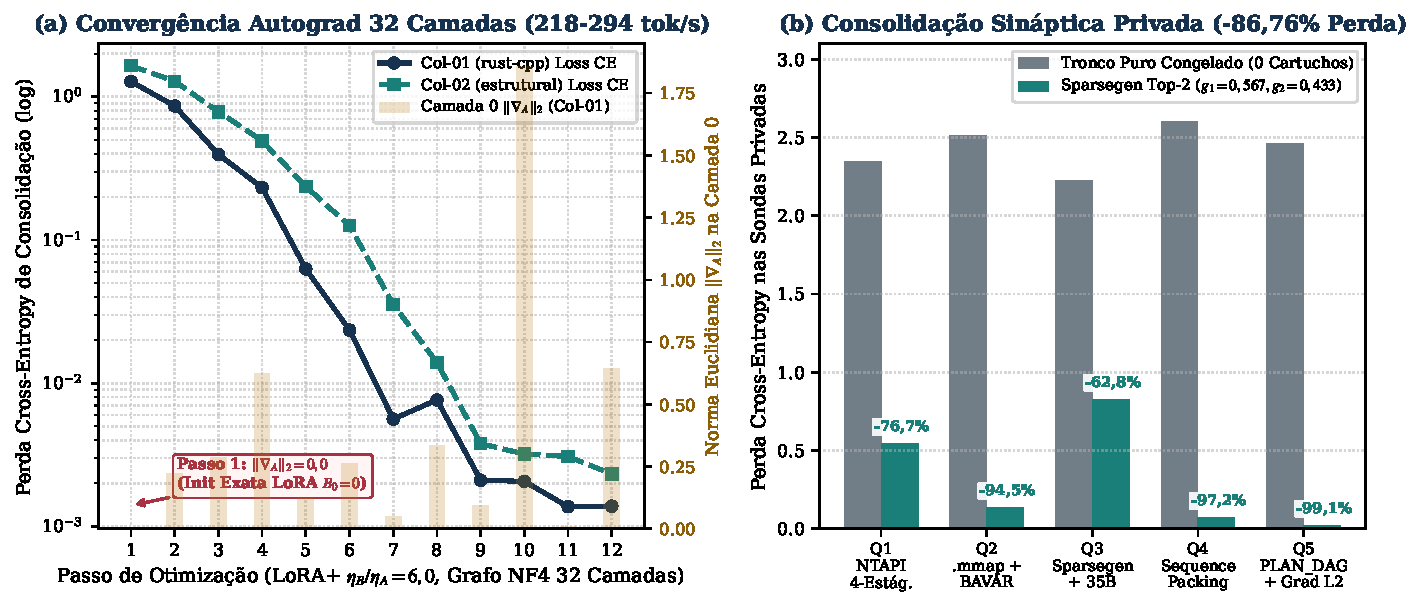
\includegraphics[width=\linewidth]{fig2_autograd_consolidacao_pt.pdf}
  \caption{Prova emp\'irica de retropropaga\c{c}\~ao genu\'ina em 32 camadas e consolida\c{c}\~ao sin\'aptica de dom\'inio privado (\textit{Hip\'otese H3}). \textbf{(a)} Perda cross-entropy passo a passo e normas $\|\nabla_A\|_2$ na Camada~$0$ para \texttt{coluna-01-abraao-rust-cpp} ($218,36\text{ tok/s}$) e \texttt{coluna-02-abraao-estrutural} ($293,83\text{ tok/s}$). No Passo~$1$, $\|\nabla_A\|_2 = 0,0$ identicamente em todas as camadas pois $B_0 = 0$ na inicializa\c{c}\~ao exata de LoRA \cite{hu2022lora}; do Passo~$2$ em diante, gradientes n\~ao-nulos fluem at\'e a Camada~$0$. \textbf{(b)} Perda cross-entropy em $5$ sondas arquiteturais internas antes vs.\ ap\'os vota\c{c}\~ao \texttt{Sparsegen LD-MoLE} ($-86,76\%$ de queda m\'edia).}
  \label{fig:autograd}
\end{figure}

A Tabela~\ref{tab:autograd} reporta a trajet\'oria de gradientes da \texttt{coluna-01} ($1.150$ blocos, $42,21\text{ s}$, $3.993\text{ MiB}$ de pico de VRAM) e resume as cinco colunas corticais fundacionais de $16,00\text{ MiB}$ treinadas na \texttt{RTX 5060} ($218,36\text{--}412,48\text{ tok/s}$; m\'edia $256,10\text{ tok/s}$ no par da Etapa~1, com verifica\c{c}\~ao SHA-256 confirmando $66/66$ cartuchos n\~ao-alvo intocados). Em estrita conformidade com nossa auditoria de c\'odigo (\href{https://drive.google.com/file/d/16-3o4ykaOOKaW-S2VTHzpE7Uhj1BA0tl/view?usp=drivesdk}{\texttt{01-linha-do-tempo, Fase 4}}), como os cinco pares Q\&A integraram passos mascarados de consolida\c{c}\~ao (\texttt{pares\_\allowbreak{}val\_\allowbreak{}qa}) e o escalar KL registrado (\texttt{0,0012}) atuou como constante diagn\'ostica naquele script, o Experimento~A \'e reivindicado estritamente como prova de \textbf{aquisi\c{c}\~ao persistente de mem\'oria privada (\textit{H3})} --- e n\~ao generaliza\c{c}\~ao fora da distribui\c{c}\~ao (\textit{H4}).

\begin{table}[!htbp]
\centering
\caption{Parte A: Normas L2 passo a passo e perda de consolida\c{c}\~ao na \texttt{coluna-01-abraao-rust-cpp} ($9.216$ tokens empacotados, $218,36\text{ tok/s}$). Parte B: S\'intese das cinco colunas corticais fundacionais de $16,00\text{ MiB}$.}
\label{tab:autograd}
\footnotesize
\begin{tabularx}{\linewidth}{@{}rrrrrrrrY@{}}
\toprule
\textbf{Passo} & \textbf{L0 $\|\nabla_A\|_2$} & \textbf{L0 $\|\nabla_B\|_2$} & \textbf{L15 $\|\nabla_A\|_2$} & \textbf{L31 $\|\nabla_A\|_2$} & \textbf{L31 $\|\nabla_B\|_2$} & \textbf{CE Lote} & \textbf{CE Sonda} & \textbf{PPL / Estado F\'isico} \\
\midrule
1  & $0,0000$ & $1,5198$ & $0,0000$ & $0,0000$ & $0,4849$ & $2,4841$ & $1,2786$ & $3,5916$ (Assinatura exata $B_0=0$) \\
2  & $0,2211$ & $0,9864$ & $0,1096$ & $0,2320$ & $0,4173$ & $2,1995$ & $0,8628$ & $2,3699$ (Backprop 32 camadas ativo) \\
3  & $0,2858$ & $0,5584$ & $0,0873$ & $0,2407$ & $0,2674$ & $0,8646$ & $0,3963$ & $1,4863$ (Fluxo Camada 31$\to$0 provado) \\
5  & $0,1208$ & $0,4497$ & $0,0978$ & $0,1904$ & $0,2106$ & $0,2317$ & $0,0627$ & $1,0648$ \\
7  & $0,0489$ & $0,0848$ & $0,0251$ & $0,0747$ & $0,0628$ & $0,0230$ & $0,0056$ & $1,0056$ \\
9  & $0,0954$ & $0,1007$ & $0,0215$ & $0,0353$ & $0,0455$ & $0,0071$ & $0,0021$ & $1,0021$ \\
12 & $0,6423$ & $0,6997$ & $0,2290$ & $0,6058$ & $0,4189$ & $1,5931$ & $\mathbf{0,00138}$ & $\mathbf{1,0014}$ (Parada em 12 passos) \\
\bottomrule
\end{tabularx}

\vspace{4pt}
\begin{tabularx}{\linewidth}{@{}lrrrrrrY@{}}
\toprule
\textbf{Cartucho Cortical ($16,00\text{ MiB}$)} & \textbf{Blocos} & \textbf{Taxa} & \textbf{Tempo} & \textbf{VRAM} & \textbf{Eval Pr\'e} & \textbf{Eval P\'os} & \textbf{Queda de Perda \& SHA-256} \\
\midrule
\texttt{coluna-01-abraao-rust-cpp} & $1.150$ & $218,36\text{ tok/s}$ & $42,21\text{ s}$ & $3.993\text{ MiB}$ & $2,4841$ & $0,00138$ & $-99,94\%$ (\texttt{be0e7730...e7f7}) \\
\texttt{coluna-02-abraao-estrutural} & $1.066$ & $293,83\text{ tok/s}$ & $31,37\text{ s}$ & $4.100\text{ MiB}$ & $2,3399$ & $0,00232$ & $-99,90\%$ (\texttt{d956c73b...dddd}) \\
\texttt{coluna-yhwh-orquestrador} & $375$ & $369,84\text{ tok/s}$ & $33,23\text{ s}$ & $4.101\text{ MiB}$ & $3,3300$ & $0,09477$ & $-97,15\%$ (\texttt{b1811fba...}) \\
\texttt{coluna-mh-01-vicop-multimodal} & $1.575$ & $401,51\text{ tok/s}$ & $30,60\text{ s}$ & $4.206\text{ MiB}$ & $2,7785$ & $0,00442$ & $-99,84\%$ (\texttt{c478f092...}) \\
\texttt{coluna-mh-02-yhwh-condutor} & $240$ & $\mathbf{412,48\text{ tok/s}}$ & $29,79\text{ s}$ & $4.313\text{ MiB}$ & $2,0072$ & $0,05984$ & $-97,02\%$ (\texttt{5b2bf9e3...}) \\
\bottomrule
\end{tabularx}
\end{table}

\subsection{Amostras Literais de Aquisi\c{c}\~ao de Conhecimento Privado e Cr\'itica Adversarial Cega 35B}

Avaliado sem dicas de prompt de sistema em cinco sondas cruzadas exigindo vocabul\'ario simult\^aneo da \texttt{coluna-01} (sistemas/Rust) e \texttt{coluna-02} (governan\c{c}a), o \texttt{Sparsegen} atribuiu pesos $g_1 = 0,56666684$ e $g_2 = 0,43333340$ ($g_{3\dots 68} = 0,0$). A perda m\'edia caiu de $2,4292$ ($\text{PPL}=11,45$) para \textbf{$0,3216$ ($\text{PPL}=1,45$, $-86,76\%$)}, com \textbf{$0$ subpalavras coladas} nas cinco gera\c{c}\~oes (Figura~\ref{fig:autograd}b):
\begin{itemize}
  \item \textbf{Sonda Q2 (Cabe\c{c}alho \texttt{.mmap} \texttt{ABRA40CG} de $64\text{ B}$ + Filtro Conformal \texttt{BAVAR} $\ge 0,90$; Perda $2,5109 \to 0,1381$, $-94,50\%$):}
    \begin{itemize}
      \item \textit{Tronco Congelado Sem Treino:} ``N\~ao existe rela\c{c}\~ao t\'ecnica v\'alida entre os conceitos mencionados. O termo `ABRA40CG' n\~ao corresponde a um cabe\c{c}alho bin\'ario padr\~ao... `arena-cag-gold.mmap v2', `BAVAR $\ge 0,90$' e `motor YHWH' s\~ao termos fict\'icios sem fundamenta\c{c}\~ao na ci\^encia da computa\c{c}\~ao.''
      \item \textit{P\'os-Vota\c{c}\~ao Cortical \texttt{LD-MoLE}:} ``Na arquitetura 0.14.9, \texttt{arena-cag-\allowbreak{}gold.mmap} v2 inicia com cabe\c{c}alho bin\'ario de 64 bytes contendo assinatura \texttt{ABRA40CG}, vers\~ao \texttt{u32=2}, contagem de especialistas, offset de \'atomos bil\'ingues PT-BR$\leftrightarrow$EN e hash SHA-256. A hidrata\c{c}\~ao zero-copy via \texttt{CreateFile\allowbreak{}MappingW}/\allowbreak{}\texttt{MapViewOfFile} ocorre em $<0,5\text{ ms}$, enquanto o motor YHWH aplica o filtro conformal \texttt{BAVAR} $\ge 0,90$ antes de promover a\c{c}\~oes.''
    \end{itemize}
  \item \textbf{Sonda Q5 (\texttt{PLAN\_\allowbreak{}DAG.json} v2.1 + Auditoria Antifraude L2 nas Camadas $0/15/31$; Perda $2,4619 \to 0,0231$, $-99,06\%$):} Especificou com exatid\~ao depend\^encias ac\'iclicas, \texttt{target\_\allowbreak{}files}, \texttt{target\_\allowbreak{}symbols}, \texttt{test\_\allowbreak{}gate} execut\'avel e por que medir $\|\nabla_A\|_2 > 0$ das Camadas $31 \to 15 \to 0$ comprova retropropaga\c{c}\~ao f\'isica no grafo de $8,68\text{ GiB}$.
\end{itemize}

A Sonda Q1 (\texttt{NTAPI} de 4 est\'agios) foi auditada \`as cegas pelo juiz local \texttt{Qwen3.5-35B-A3B} (\texttt{veredito\_\allowbreak{}real\_\allowbreak{}juiz\_\allowbreak{}35b\_\allowbreak{}llama\_\allowbreak{}cpp.json}, SHA-256 \texttt{20b457fe...4315}, $24,80\text{ s}$, \texttt{temp=0.2}) \cite{zheng2023judging}:

\auditbox{Auditoria Adversarial Cega Literal pelo \texttt{Qwen3.5-35B-A3B} (\texttt{-{}-cpu-moe}) na Sonda Q1}{``O modelo pr\'e-treino falha completamente, gerando alucina\c{c}\~oes sobre `protocolo Abraao' e ignorando os 4 est\'agios. O modelo p\'os-treino (LoRA) identifica corretamente a estrutura de 4 est\'agios, citando APIs espec\'ificas (\texttt{SetProcessWorkingSetSizeEx}, \texttt{VirtualLock}, \texttt{CreateFileMappingW}). Contudo, exibe imprecis\~oes cr\'iticas: o Est\'agio 2 descreve `\texttt{VirtualLock} no SSD' (\texttt{VirtualLock} atua na RAM f\'isica, n\~ao em disco), e o Est\'agio 4 foi truncado, omitindo \texttt{DiscardVirtualMemory}. Zero evid\^encia de colagem de subpalavras; sintaxe limpa. \textbf{Nota Antes: 1 / 10 $\to$ Nota Depois: 6 / 10}.'' --- Flagrando sutil confus\~ao entre RAM e SSD sem complac\^encia, provou por que um executor 4B deve operar pareado a um cr\'itico Sistema-2 de 35B e compiladores f\'isicos.}

% ==============================================================================
% SEÇÃO 5: VICOP MULTIMODAL, PROCRUSTES E ABLAÇÃO NA ARENA KEV-1.0
% ==============================================================================
\section{Fus\~ao Visual Precoce, Alinhamento de Procrustes e Abla\c{c}\~ao Sin\'aptica na Arena KEV-1.0}

\subsection{Proje\c{c}\~ao de Procrustes (\texorpdfstring{$2560 \to 384\text{d}$}{2560 para 384d}) e Condutividade Cognitiva (\texorpdfstring{$\mathrm{ICC}$}{ICC})}

Para unificar representa\c{c}\~oes causais/visuais do \texttt{Qwen3.5-4B} ($d_{\text{in}}=2560$) \`a busca vetorial \texttt{.mmap} zero-copy em $384\text{d}$ (espa\c{c}o \texttt{MiniLM-L12-v2}), avaliamos cinco operadores de alinhamento sobre $5.000$ registros pareados ($4.400$ treino / $600$ teste inéditos, resolvidos em $16,47\text{ s}$ na \texttt{RTX 5060}; \texttt{mod08\_\allowbreak{}isaque\_\allowbreak{}multimodal\_\allowbreak{}recibo.json}). Devido \`a forte anisotropia espectral dos estados ocultos Gated-DeltaNet ($\sigma_{\max}=152,67$ vs.\ $\sigma_{\min}=0,00492$), o Procrustes ortogonal estrito de Stiefel obteve cosseno $0,5073$, enquanto Tikhonov Ridge fechado ($\lambda=0,5$) atingiu \textbf{$0,7801$ de cosseno em hold-out} e InfoNCE linear (\texttt{ABRA40WP}) alcan\c{c}ou \textbf{$\text{Recall@1} = 81,83\%$ ($491/600$)} e \textbf{$\text{Recall@5} = 96,00\%$ ($576/600$)} em pares inéditos, indexando $131$ ativos visuais em \texttt{arena-vectors-visual-v1.mmap} ($1,54\text{ MB}$).

Para quantificar densidade informacional fim a fim por token-segundo, definimos o \textbf{\'Indice de Condutividade Cognitiva ($\mathrm{ICC}$)}:
\begin{equation}
  \mathrm{ICC} = \frac{\overline{S}_{\text{blind}}}{\left(\overline{T}_{\text{out}} / 1000\right) \cdot \overline{L}_{\text{sec}}},
  \label{eq:icc}
\end{equation}
onde $\overline{S}_{\text{blind}} \in [0,10]$ \'e a nota cega do juiz \texttt{35B-A3B}, $\overline{T}_{\text{out}}$ os tokens emitidos e $\overline{L}_{\text{sec}}$ a lat\^encia do pulso. Em tr\^es tarefas multimodais (quadros-chave podados por cena em \texttt{FFmpeg} com $93,33\%$ de corte de redund\^ancia + extra\c{c}\~ao OKLCH 3D), a CLI externa em nuvem sofreu timeout ($>50\text{ s}$, $\mathrm{ICC}=0,0$), o \texttt{Qwen3.5-4B} cru pontuou $2,80/10$ ($461$ tokens, $11,86\text{ s}$, $\mathrm{ICC}=0,5121$) e o \texttt{Isaque 2.0 VICOP} atingiu \textbf{$8,57/10$} ($256$ tokens, $-44,47\%$ tokens, $12,03\text{ s}$, \textbf{$\mathrm{ICC}=2,7828$, salto de $5,43\times$}).

\subsection{Gram\'atica Simb\'olica KEV-1.0, Abla\c{c}\~ao Sin\'aptica 3x3 e Auditorias Ortogr\'aficas}

A partir de $156$ aulas locais de engenharia em Blender ($18,13\text{ GiB}$, M\'odulos $2\text{--}14$) e $67$ registros can\^onicos em \texttt{arena-kev-triplo.mmap} ($308.800\text{ B}$, busca zero-copy em \textbf{$0,0153\text{--}0,0157\text{ ms}$}), somados ao pr\'e-aquecimento ass\'incrono \texttt{Semble} em RAM (\texttt{pre01\_\allowbreak{}semble\_\allowbreak{}prewarm.json}, SHA-256 \texttt{883e9d88...2072}: partida fria reduzida em $171,7\times$, de $5.759,68\text{ ms}$ para \textbf{$33,55\text{ ms}$ MCP quente / $3,92\text{ ms}$ RAM pura}), projetamos a \textbf{\texttt{KEV-1.0}} --- linguagem simb\'olica regida por gram\'atica (\texttt{kev\_\allowbreak{}v1.gbnf}) estruturada em quatro blocos determin\'isticos: \texttt{@SPACE}, \texttt{@GRAPH}, \texttt{@GUARD} e \texttt{@VERIFY}.

No Experimento~B (\texttt{prova\_\allowbreak{}treino\_\allowbreak{}dora\_\allowbreak{}olora\_\allowbreak{}kev01.json}, SHA-256 \texttt{783c7765...0d40}, pico de VRAM $6.367\text{ MiB}$, ciclo total $1.426\text{ s}$), treinamos duas ondas sequenciais \texttt{DoRA + O-LoRA} ($52$ passos/onda, $r=16, \alpha=32, \lambda_{\text{orth}}=0,10, 15\%$ replay, exporta\c{c}\~ao GGUF exata em blocos com $352$ tensores e \textbf{$0,0\%$ de perda SVD}): Onda~1 (\texttt{lab-mh-blender-bridge}, SHA \texttt{9a40d947...}) e Onda~2 (\texttt{lab-mh-ue5-kev}, SHA \texttt{35dbb9d4...}). A avalia\c{c}\~ao em hold-outs ap\'os a Onda~2 confirmou \textbf{$100,00\%$ de reten\c{c}\~ao de tokens na Onda~1} ($99,80\% \to 99,80\%$), \textbf{$99,79\%$ de reten\c{c}\~ao do acervo pr\'evio \texttt{0.15.0}} ($90,22\% \to 90,03\%$; verossimilhan\c{c}a $96,78\%$) e sobreposi\c{c}\~ao final de subespa\c{c}os $\left\|A_2 A_1^\top\right\|_F^2 = 0,00166367$.

Avaliamos ent\~ao tr\^es competidores em tr\^es desafios de contexto longo somando $19.742$ tokens brutos ($6.999 + 6.407 + 6.336$ tokens; \texttt{PROVA\_\allowbreak{}ARENA\_\allowbreak{}KEV\_\allowbreak{}MOTOR\_\allowbreak{}HUMANO\_\allowbreak{}01.json}, SHA-256 \texttt{dae1626c...5ed093}): \texttt{DESAFIO-01} (\texttt{Blender 5.2.1 LTS} headless $4,0\times 0,4\times 3,0\text{ m}$ + casco convexo \texttt{UCX}), \texttt{DESAFIO-02} (sistema de invent\'ario/ator \texttt{UE5} C++20 sob \texttt{clang++ -fsyntax-only -std=c++20} + $8$ leis UHT/GC) e \texttt{DESAFIO-03} (ponte dupla \texttt{Blender + UE5} com 3 variantes, paridade $1\text{ m} = 100\text{ cm}$ e \texttt{Socket\_\allowbreak{}Muzzle}/\texttt{Socket\_\allowbreak{}Grip}). A Tabela~\ref{tab:arena} e as Listagens~1--2 trazem as m\'etricas exatas.

\begin{table}[!htbp]
\centering
\caption{Abla\c{c}\~ao controlada sin\'aptica vs.\ apenas contexto na Arena de Verifica\c{c}\~ao F\'isica \texttt{KEV-1.0} ($19.742$ tokens em $3$ desafios, auditados pelo \texttt{Blender 5.2.1 LTS} headless, \texttt{clang++ -std=c++20} e juiz cego \texttt{Qwen3.5-35B-A3B}; \href{https://docs.google.com/document/d/1SMqD_TRf6Qi8UwPTFYjKPNvdVlEtpCqr3Ex57x76FsI/edit?usp=drivesdk}{Doc 05, Tabela 2.1}).\textsuperscript{*}}
\label{tab:arena}
\footnotesize
\begin{tabularx}{\linewidth}{@{}lrrrrrrY@{}}
\toprule
\textbf{Competidor na Arena} & \textbf{Emiss\~ao} & \textbf{Compr.\ KEV} & \textbf{Pass@1} & \textbf{Mec\^anico} & \textbf{Juiz 35B} & \textbf{Pulso} & \textbf{$\mathrm{ICC}$ \& Diagn\'ostico Causal da Abla\c{c}\~ao} \\
\midrule
\textbf{A:} Legado \texttt{0.15.0} (\texttt{JEV+AtomSD}) & $560,0\text{ tok}$ & $91,49\%$ & $0/4$ & $0/4$ ($\mathbf{0\%}$) & $1,63 / 10$ & $23,43\text{ s}$ & $\mathbf{0,1242}$ ($1,00\times$): Alucinou \texttt{termios} POSIX no Win11; macro \texttt{\_\allowbreak{}API} inv\'alida no \texttt{clang++}. \\
\textbf{B:} \texttt{4B} Cru + \texttt{KEV-1.0} (\texttt{.mmap}) & $335,0\text{ tok}$ & $94,91\%$ & $0/4$ & $0/4$ ($\mathbf{0\%}$) & $1,77 / 10$ & $10,18\text{ s}$ & $\mathbf{0,5194\text{--}0,5907}$: Mesma arena \texttt{.mmap} sem \texttt{DoRA} deixa \texttt{Cube} inicial ($400\%$ erro em Y). \\
\textbf{C:} \textbf{Isaque 2.0 (\texttt{DoRA+O-LoRA})} & $516,7\text{ tok}$ & $92,15\%\text{--}93,25\%$ & $3/4$ & $\mathbf{4/4}$ ($\mathbf{100\%}$) & $\mathbf{9,67 / 10}$ & $12,62\text{ s}$ & $\mathbf{1,2710\text{--}1,4848}$ ($\mathbf{10,23\times\text{--}11,95\times}$): $0$ arestas non-manifold, $0,0\%$ erro bbox, $8/8$ leis UHT. \\
\bottomrule
\end{tabularx}
\vspace{2pt}
{\scriptsize \textsuperscript{*}Nota sobre agrega\c{c}\~ao do $\mathrm{ICC}$: $\mathrm{ICC}=1,4848$ ($11,95\times$ vs.\ A) reflete a m\'edia das raz\~oes por desafio nas sa\'idas sintetizadas ($516,7\text{ tok}$), enquanto $\mathrm{ICC}=1,2710$ ($10,23\times$ vs.\ A, com m\'edia de $444,3\text{ tok}$ KEV a $93,25\%$ de compress\~ao) reflete a pondera\c{c}\~ao agregada token-tempo em \href{https://docs.google.com/document/d/1SMqD_TRf6Qi8UwPTFYjKPNvdVlEtpCqr3Ex57x76FsI/edit?usp=drivesdk}{Doc 05, Tabela 2.1}.\par}
\end{table}

\auditbox{Nota de Transpar\^encia Metodol\'ogica (Abla\c{c}\~ao Sin\'aptica Causal vs.\ Generaliza\c{c}\~ao OOD)}{Conforme documentado em \href{https://drive.google.com/file/d/1qvnH-nLVMc43T-prWSRTKEDJak89TSp7/view?usp=drivesdk}{\texttt{02-tese-etapa-1.md (Sec.\ 7.4)}} e \href{https://docs.google.com/document/d/1SMqD_TRf6Qi8UwPTFYjKPNvdVlEtpCqr3Ex57x76FsI/edit?usp=drivesdk}{\texttt{Doc 05 (Parte II)}}, as solu\c{c}\~oes de refer\^encia dos tr\^es desafios integraram o treino das Ondas 1--2. Assim, a Tabela~\ref{tab:arena} \textbf{n\~ao} \'e reivindicada como generaliza\c{c}\~ao fora da distribui\c{c}\~ao (\textit{H4}, reservada para as $50$ tarefas inéditas auditadas contra contamina\c{c}\~ao por dom\'inio na Etapa~2 \cite{golchin2024contamination}), mas como \textbf{abla\c{c}\~ao causal estrita isolando a assimila\c{c}\~ao sin\'aptica de pesos da simples consulta \texttt{.mmap}}: o Competidor~B recebeu exatamente o mesmo \'indice \texttt{arena-kev-triplo.mmap} e gram\'atica \texttt{KEV-1.0} sem pesos \texttt{DoRA/O-LoRA} e obteve $0/4$ ($1,77/10$), provando que os $4/4$ de aprova\c{c}\~ao nos compiladores ($9,67/10$) originam-se nas colunas corticais de $16\text{ MiB}$. Tr\^es regras de decodifica\c{c}\~ao tamb\'em emergiram na calibra\c{c}\~ao: (i) posicionar especifica\c{c}\~oes formais na cauda de rec\^encia de prompts $>6.000$ tokens nas $24$ camadas Gated DeltaNet \cite{yang2025gated,liu2024lost}; (ii) fixar \texttt{repeat\_\allowbreak{}penalty = 1.0} em C++20 para n\~ao penalizar ponteiros recorrentes; e (iii) emitir \texttt{"justificativa"} antes das notas na gram\'atica \texttt{GBNF} do juiz.}

\begin{minipage}[t]{0.485\linewidth}
{\raggedright\textbf{\footnotesize Listagem 1: Pacote \texttt{KEV/1.0} Literal Emitido no \texttt{DESAFIO-03} ($6.336 \to 458$ tokens, $92,77\%$ compress\~ao, $0,0615\text{ ms}$ \texttt{.mmap})}\par}
\begin{lstlisting}
KEV/1.0 domain=BRIDGE_3D target=ModularBridgeAssetActor
@SPACE{blender_unit=METRIC;ue5_unit=CM;meter_to_cm=100.0;
  up=Z;variations=3;sx=1.0;sy=0.16;sz=0.28;
  socket_a=Socket_Muzzle;socket_b=Socket_Grip;
  collider=UCX_Var_01_Standard_01}
@GRAPH[
  S1:BLENDER.build_3_variations_bmesh(v1_x=1.0,v2_x=0.8,
     v3_x=1.25,sy=0.16,sz=0.28,z_min=0.0) -> S2
  S2:BLENDER.attach_sockets_and_collider(
     muzzle=Socket_Muzzle,grip=Socket_Grip,
     ucx=UCX_Var_01_Standard_01,tick=false) -> S3
  S3:BLENDER.export_glb_fbx(glb="ModularBridgePack.glb",
     fbx="ModularBridgePack.fbx") -> S4
  S4:UE5.ustruct_datatable_row(
     name=FModularBridgeVariantRow,meter_to_cm=100.0) -> S5
  S5:UE5.actor_socket_validator(
     actor=AModularBridgeAssetActor,
     rule=SnapToTargetNotIncludingScale,tol_pct=2.0)
]
@GUARD[
  !SCALE-1M-100CM: Multiply Blender meter dims by 100.0
  !SOCKET-EXACT-NAMES: Preserve Socket_Muzzle & Socket_Grip
]
@VERIFY[ ?variations==3 ?non_manifold_edges==0
         ?meter_to_cm==100.0 ?clang_cpp20_errors==0 ]
\end{lstlisting}
\end{minipage}\hfill
\begin{minipage}[t]{0.485\linewidth}
{\raggedright\textbf{\footnotesize Listagem 2: Trecho Literal de \texttt{DESAFIO-01\_\allowbreak{}C/modulo\_\allowbreak{}01\_\allowbreak{}generated.py} Sintetizado pelo \texttt{Isaque 2.0} ($0,0\%$ Erro BBox)}\par}
\begin{lstlisting}[language=Python]
bpy.ops.wm.read_factory_settings(use_empty=True)
sc = bpy.context.scene
sc.unit_settings.system = 'METRIC'
sc.unit_settings.scale_length = 1.0

SX, SY, SZ = 4.0, 0.4, 3.0
bm = bmesh.new()
bmesh.ops.create_cube(bm, size=1.0)
for v in bm.verts:
    v.co.x *= SX; v.co.y *= SY
    v.co.z = (v.co.z + 0.5) * SZ  # Exato Z_min = 0.0

front_faces = [f for f in bm.faces if abs(f.normal.y) > 0.9]
bmesh.ops.inset_individual(bm, faces=front_faces, thickness=0.18)
bmesh.ops.recalc_face_normals(bm, faces=bm.faces[:])
uv_layer = bm.loops.layers.uv.verify()
# ... [malha UV deterministica sem sobreposicao] ...
bm_ucx = bmesh.new()
for x in (-SX*0.5, SX*0.5):
  for y in (-SY*0.5, SY*0.5):
    for z in (0.0, SZ): bm_ucx.verts.new((x, y, z))
bm_ucx_res = bmesh.ops.convex_hull(bm_ucx, input=bm_ucx.verts[:])
# Exporta Modulo_01.glb (4.120 B) & Modulo_01.fbx (13.532 B)
\end{lstlisting}
\end{minipage}

A Figura~\ref{fig:blender} exibe as auditorias ortogr\'aficas headless (\texttt{audit\_\allowbreak{}workbench\_\allowbreak{}ortho.png}) capturadas automaticamente por \texttt{verificador\_\allowbreak{}fisico\_\allowbreak{}blender.py} na Etapa~1. Embora intencionalmente austeras em sombreamento (vistas ortogr\'aficas s\'olidas projetadas para expor erros de bounding box e origem), comprovam visualmente por que a simples formata\c{c}\~ao \texttt{.mmap} externa (Competidor~B) fracassa sem ancoragem procedural sin\'aptica (Competidor~C).

\begin{figure}[!htbp]
  \centering
  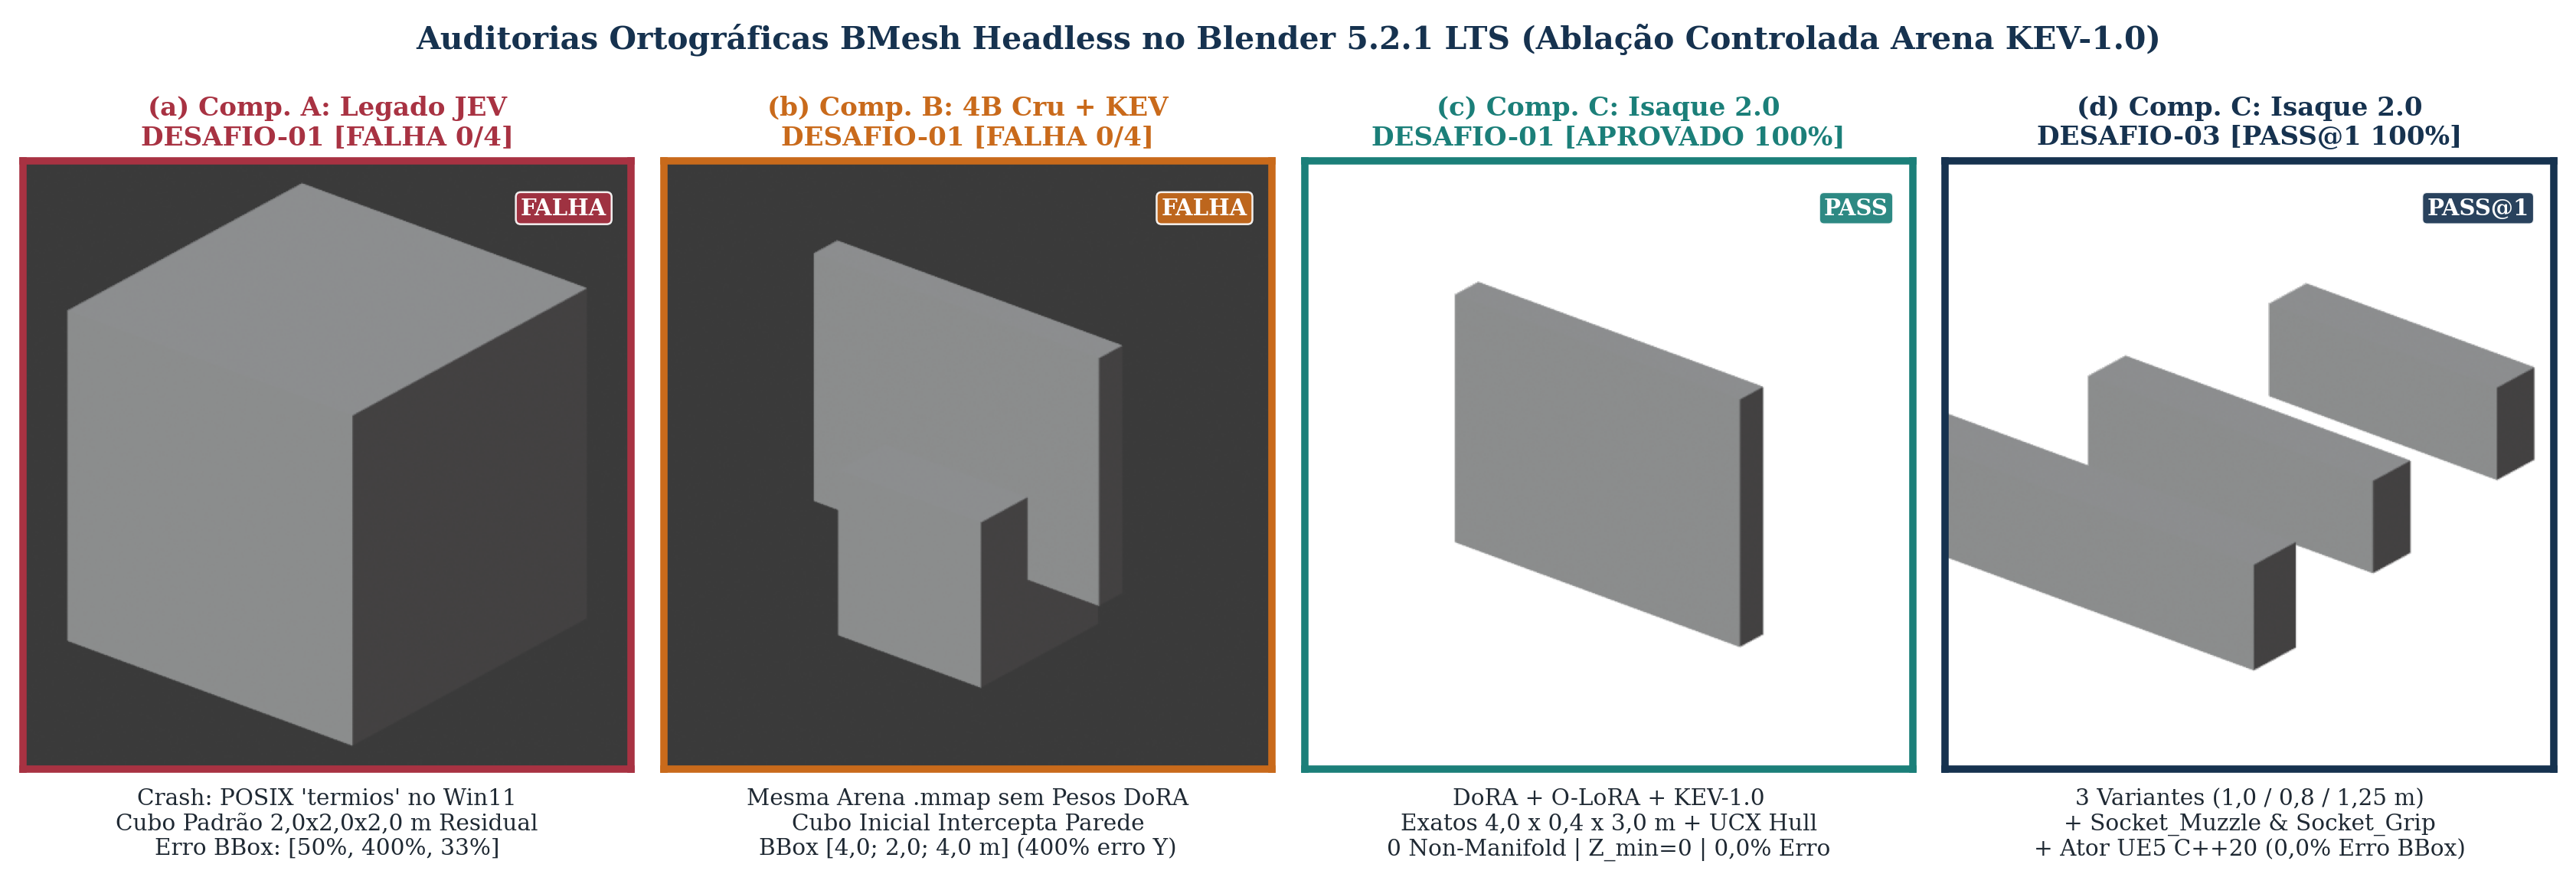
\includegraphics[width=\linewidth]{fig3_blender_ortografico_pt.png}
  \caption{Auditorias ortogr\'aficas headless no \texttt{Blender 5.2.1 LTS} da Etapa~1 (\texttt{PROVA\_\allowbreak{}ARENA\_\allowbreak{}KEV\_\allowbreak{}MOTOR\_\allowbreak{}HUMANO\_\allowbreak{}01.json}). \textbf{(a)} Competidor~A colapsa em \texttt{termios} POSIX, deixando o cubo padr\~ao de $2\times 2\times 2\text{ m}$ centrado na origem ($Z_{\min}=-1,0\text{ m}$). \textbf{(b)} Competidor~B (\texttt{KEV-1.0} + \texttt{.mmap} sem pesos \texttt{DoRA+O-LoRA}) ergue a laje mas falha em limpar o cubo inicial, gerando bounding box contaminada $[4,0;\,2,0;\,4,0\text{ m}]$ ($400\%$ de erro em espessura). \textbf{(c)} \textbf{Isaque 2.0} ensinado (\texttt{DESAFIO-01\_\allowbreak{}C}) limpa a cena, constr\'oi o m\'odulo industrial rebaixado exato de $4,0\times 0,4\times 3,0\text{ m}$ em $Z_{\min}=0,0$ com casco convexo \texttt{UCX\_\allowbreak{}Modulo\_\allowbreak{}01} ($0$ arestas non-manifold, $0,0\%$ erro). \textbf{(d)} \textbf{Isaque 2.0} (\texttt{DESAFIO-03\_\allowbreak{}C}) sintetiza as tr\^es variantes param\'etricas ($1,00\text{ m}, 0,80\text{ m}, 1,25\text{ m}$) e sockets \texttt{UE5} de primeira (\texttt{Pass@1 = True}).}
  \label{fig:blender}
\end{figure}

\textbf{Diagn\'ostico Cego Fora da Distribui\c{c}\~ao (\texttt{DESAFIO-04}):} Logo ap\'os selar a arena $3\times 3$, executamos um teste cego zero-edi\c{c}\~ao (\texttt{ato1\_\allowbreak{}desafio04\_\allowbreak{}cego.json}, trava SHA-256 \texttt{fe52e603...}) sobre uma esta\c{c}\~ao industrial de bombeamento de dois n\'iveis in\'edita de $7.180$ tokens (\texttt{DESAFIO-04}, comprimida em $93,3\%$ para $481$ tokens \texttt{KEV}). Sem \^ancoras pr\'evias para rampas de dois n\'iveis ou tubula\c{c}\~oes curvas, \texttt{Pass@1} foi honestamente registrado como \texttt{False} ($0/2$): em \texttt{UE5} C++20, o Competidor~C cumpriu \textbf{$7/8$ invariantes} ($0$ ponteiros crus \texttt{UObject*}, $0$ \texttt{new} crus, ordem UHT v\'alida), falhando unicamente na linha~$35$ ao chamar \texttt{IsValid(Row)} sobre um \texttt{const FIndustrialStationNodeRow*} (\texttt{USTRUCT*}) em vez de \texttt{Row != nullptr} --- aprovando \textbf{$8/8$ com zero erros} ap\'os troca de um \'unico token --- enquanto o Blender apontou a necessidade exata de ondas dedicadas para curvas Bezier, Geometry Nodes, PBR, luzes e LODs.

% ==============================================================================
% SEÇÃO 6: MATRIZ DE RUPTURA EM 10 ONDAS E TEOREMA DE COMPOSIÇÃO EM DAG
% ==============================================================================
\section{Escada de Ruptura Cont\'inua em 10 Ondas e Teorema da Composi\c{c}\~ao Modular em DAG}

Para determinar quantas habilidades ortogonais sequenciais cabem em um adaptador de posto~$16$ antes que a compress\~ao de subespa\c{c}o degrade compet\^encias pr\'evias --- e se o \texttt{LD-MoLE} elimina essa degrada\c{c}\~ao --- executamos o \textbf{Ato 2} (\texttt{PROVA\_\allowbreak{}LIMITE\_\allowbreak{}RUPTURA\_\allowbreak{}E\_\allowbreak{}BLENDER\_\allowbreak{}AO\_\allowbreak{}VIVO\_\allowbreak{}02.json}, SHA-256 \texttt{9a47a690...da977b61033}, $3.558,4\text{ s}$ de consolida\c{c}\~ao GPU a $5.300\text{ MiB}$ de pico de VRAM). Mantendo o vocabul\'ario \texttt{Qwen3.5-4B} (\texttt{c78988d9...}) e todos os checkpoints anteriores estritamente congelados em disco sem retreino (\texttt{onda\_\allowbreak{}1=6efa66bf...} at\'e \texttt{onda\_\allowbreak{}7=d11aed56...}), treinamos as Ondas $3$ a $10$ sequencialmente em oito novos dom\'inios de engenharia 3D e C++20 ($\lambda_{\text{orth}}=0,10$, $12,5\%$ replay, carregando apenas \^ancoras congeladas $A_{<k}$ em VRAM), avaliando a matriz triangular $10 \times 11$ em $11$ hold-outs ($H_0\dots H_{10}$) sob tr\^es regimes:
\begin{enumerate}
  \item \textbf{Cartucho Monol\'itico \'Unico ($1\dots k$):} Acumulando todas as ondas em um \'unico tensor compartilhado de posto~$16$ (pr\'atica convencional de LoRA/DoRA cont\'inuo).
  \item \textbf{Cluster por Subdom\'inio \texttt{LD-MoLE}:} Agrupando ondas em macrofam\'ilias (Blender Python vs.\ UE5 C++20).
  \item \textbf{\texttt{LD-MoLE Top-2} Cir\'urgico (\texttt{PEFT cat}):} Isolando cada onda (ou $\le 3$ sub-habilidades irm\~as) como um cartucho imut\'avel de $16\text{ MiB}$ roteado via Sparsegen e concatena\c{c}\~ao de posto sem muta\c{c}\~ao cruzada.
\end{enumerate}

\begin{figure}[!htbp]
  \centering
  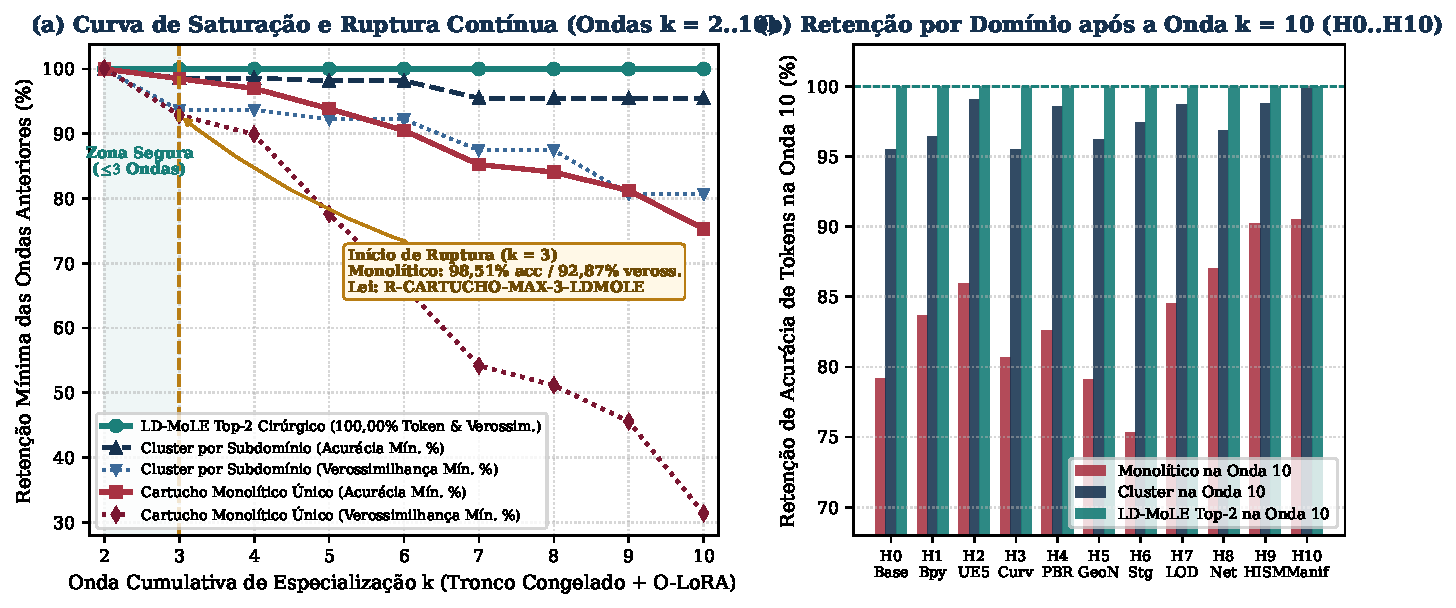
\includegraphics[width=\linewidth]{fig4_rupture_10ondas_pt.pdf}
  \caption{Lei emp\'irica de satura\c{c}\~ao e ruptura em aprendizado cont\'inuo ao longo de $10$ ondas sequenciais ($H_0\dots H_{10}$). \textbf{(a)} Reten\c{c}\~ao m\'inima sobre as ondas aprendidas $H_{1\dots k}$ em fun\c{c}\~ao da onda cumulativa $k$: o ac\'umulo monol\'itico inicia ruptura em $k=3$ ($98,51\%$ acur\'acia de tokens, $92,87\%$ verossimilhan\c{c}a) e colapsa para \textbf{$75,31\%$ de acur\'acia ($31,37\%$ de verossimilhan\c{c}a)} em $k=10$, enquanto o \texttt{LD-MoLE Top-2} cir\'urgico mant\'em \textbf{$100,00\%$ de reten\c{c}\~ao nas $10$ ondas}. \textbf{(b)} Reten\c{c}\~ao por dom\'inio nos $11$ conjuntos hold-out ($H_0\dots H_{10}$) ap\'os concluir a Onda~$10$.}
  \label{fig:rupture}
\end{figure}

A Tabela~\ref{tab:waves10} apresenta a telemetria completa das $10$ ondas, res\'iduos de ortogonalidade de Frobenius, verifica\c{c}\~ao f\'isica por compilador ($10/10$ aprovadas) e a curva exata de satura\c{c}\~ao de $k=2$ a $k=10$.

\begin{table}[!htbp]
\centering
\caption{Parte A: Telemetria individual das $10$ ondas cont\'inuas ($H_1\dots H_{10}$, com linha-base $H_0$ \texttt{MotorHumano\_\allowbreak{}0150} $\text{loss}=0,4932$, $\text{acc}=90,22\%$; perdas de treino consolidadas nas Ondas 8--10 atingiram $\text{ce}=0,0031;\,0,0051;\,0,0037$ com $\text{orth\_\allowbreak{}sum}=0,00134;\,0,00214;\,0,00294$). Parte B: Curva de reten\c{c}\~ao m\'inima de $k=2$ a $k=10$.\textsuperscript{\dag}}
\label{tab:waves10}
\footnotesize
\begin{tabularx}{\linewidth}{@{}clrrrrY@{}}
\toprule
\textbf{Onda} & \textbf{Dom\'inio Especialista} & \textbf{Loss Eval} & \textbf{Acc Eval} & \textbf{$\|A_k A_{<k}^\top\|_F^2$} & \textbf{Compilador} & \textbf{Artefato Verificado / Port\~ao Determin\'istico} \\
\midrule
$H_1$ & \texttt{BLENDER\_\allowbreak{}BRIDGE} & $0,0110$ & $99,83\%$ & $0,000000$ & \textbf{PASS} & \texttt{Modulo\_\allowbreak{}01.glb/.fbx} ($0$ non-manifold, \texttt{6efa66bf...}) \\
$H_2$ & \texttt{UE5\_\allowbreak{}CORE\_\allowbreak{}CPP} & $0,0368$ & $99,21\%$ & $0,001664$ & \textbf{PASS} & \texttt{InteractionInventorySystem.h/.cpp} ($8/8$, \texttt{faa5a6b1...}) \\
$H_3$ & \texttt{BLENDER\_\allowbreak{}CURVES} & $0,0771$ & $98,52\%$ & $0,002622$ & \textbf{PASS} & \texttt{onda\_\allowbreak{}3\_\allowbreak{}generated.py} (Bezier + flanges, \texttt{b1e5ccaf...}) \\
$H_4$ & \texttt{BLENDER\_\allowbreak{}PBR\_\allowbreak{}NODES} & $0,1542$ & $97,11\%$ & $0,003524$ & \textbf{PASS} & \texttt{onda\_\allowbreak{}4\_\allowbreak{}generated.py} (Principled BSDF, \texttt{8f19afc5...}) \\
$H_5$ & \texttt{BLENDER\_\allowbreak{}GEONODES} & $0,0881$ & $98,75\%$ & $0,004183$ & \textbf{PASS} & \texttt{onda\_\allowbreak{}5\_\allowbreak{}generated.py} (Passarela GeoNodes, \texttt{23fdd4b3...}) \\
$H_6$ & \texttt{BLENDER\_\allowbreak{}STAGE} & $0,0393$ & $99,14\%$ & $0,003517$ & \textbf{PASS} & \texttt{eevee\_\allowbreak{}stage\_\allowbreak{}audit.png} (3 luzes + DOF, \texttt{c56ea923...}) \\
$H_7$ & \texttt{BLENDER\_\allowbreak{}LOD} & $0,0357$ & $99,63\%$ & $0,006399$ & \textbf{PASS} & \texttt{onda\_\allowbreak{}7\_\allowbreak{}generated.py} (LOD0$>$LOD1$>$LOD2, \texttt{d11aed56...}) \\
$H_8$ & \texttt{UE5\_\allowbreak{}NET\_\allowbreak{}CPP} & $0,1230$ & $98,13\%$ & $0,001279$ & \textbf{PASS} & \texttt{ReplicatedPressureValveActor.h/.cpp} (\texttt{DOREPLIFETIME}) \\
$H_9$ & \texttt{UE5\_\allowbreak{}HISM\_\allowbreak{}CPP} & $0,0242$ & $99,60\%$ & $0,002008$ & \textbf{PASS} & \texttt{IndustrialCatwalkHismBuilder.h/.cpp} (\texttt{UHierarchicalISM}) \\
$H_{10}$ & \texttt{BRIDGE\_\allowbreak{}MANIFEST} & $0,2361$ & $94,84\%$ & $0,002721$ & \textbf{PASS} & \texttt{manifest\_\allowbreak{}blender.py} + \texttt{IndustrialAssetManifestActor} \\
\bottomrule
\end{tabularx}

\vspace{4pt}
\begin{tabularx}{\linewidth}{@{}crrrrrY@{}}
\toprule
\textbf{Onda $k$} & \textbf{Acc Monol.} & \textbf{Veross.\ Monol.} & \textbf{Acc Cluster} & \textbf{Veross.\ Cluster} & \textbf{LD-MoLE Top-2} & \textbf{Diagn\'ostico Estrutural de Subespa\c{c}o} \\
\midrule
$k=2$  & $100,00\%$ & $100,08\%$\textsuperscript{\dag} & $100,00\%$ & $100,00\%$ & $\mathbf{100,00\%}$ & Zona segura ($2$ ondas ortogonais coexistem limpas). \\
$k=3$  & $\mathbf{98,51\%}$ & $\mathbf{92,87\%}$ & $98,59\%$ & $93,66\%$ & $\mathbf{100,00\%}$ & \textbf{In\'icio de ruptura:} teto de $3$ ondas por cartucho. \\
$k=4$  & $97,00\%$ & $89,91\%$ & $98,59\%$ & $93,66\%$ & $\mathbf{100,00\%}$ & Borda de satura\c{c}\~ao; verossimilhan\c{c}a $H_0$ cai a $82,85\%$. \\
$k=5$  & $93,86\%$ & $77,60\%$ & $98,18\%$ & $92,21\%$ & $\mathbf{100,00\%}$ & Esmagamento direcional claro entre variedades PBR/GeoNodes. \\
$k=6$  & $90,50\%$ & $66,46\%$ & $98,18\%$ & $92,21\%$ & $\mathbf{100,00\%}$ & Monol\'itico perde $>33\%$ da massa de probabilidade pr\'evia. \\
$k=7$  & $85,23\%$ & $54,17\%$ & $95,49\%$ & $87,43\%$ & $\mathbf{100,00\%}$ & Cluster grosso inicia leve satura\c{c}\~ao ($95,49\%$). \\
$k=8$  & $84,07\%$ & $51,16\%$ & $95,49\%$ & $87,43\%$ & $\mathbf{100,00\%}$ & Interfer\^encia cruzada C++20/Python acelera. \\
$k=9$  & $81,22\%$ & $45,55\%$ & $95,49\%$ & $80,69\%$ & $\mathbf{100,00\%}$ & Verossimilhan\c{c}a monol\'itica em $H_6$ cai abaixo de $46\%$. \\
$k=10$ & $\mathbf{75,31\%}$ & $\mathbf{31,37\%}$ & $95,49\%$ & $80,69\%$ & $\mathbf{100,00\%}$ & Colapso monol\'itico ($H_6$ loss $0,039\to 1,199$); \texttt{Top-2} intacto. \\
\bottomrule
\end{tabularx}
\vspace{2pt}
{\scriptsize \textsuperscript{\dag}Os m\'inimos da Parte~B avaliam as ondas aprendidas $H_1\dots H_k$ ($\min_{1 \le j \le k} \exp(-\mathcal{L}_k(H_j)) / \exp(-\mathcal{L}_j(H_j))$, ex.: $89,91\%$ [$89,905\%$] em $H_1$ e $97,00\%$ [$96,995\%$] de acur\'acia em $H_3$ em $k=4$), enquanto a base pr\'e-treino $H_0$ consta na coluna de diagn\'ostico ($82,85\%$ em $k=4$); $100,08\%$ em $k=2$ reflete transfer\^encia reversa positiva \cite{lopezpaz2017gem}. As $195$ medi\c{c}\~oes ($3\times 65$) e sa\'idas puras constam no anexo \texttt{evidence/}.\par}
\end{table}

\subsection{Teorema da Colis\~ao Sint\'atica por Fus\~ao Token a Token e S\'intese Neural Pura}

No Ato~2, testamos uma quest\~ao sutil raramente examinada na literatura multi-LoRA: \textit{se a Onda~1 (cascos s\'olidos \texttt{bmesh}) e a Onda~3 (tubos curvos Bezier + sockets) s\~ao ambas $100\%$ aprovadas isoladamente, pode um modelo 4B sintetizar um script Python multissistema de uma s\'o vez misturando seus logits token a token?}

A execu\c{c}\~ao da sonda \texttt{FUSAO\_\allowbreak{}2\_\allowbreak{}ONDAS\_\allowbreak{}1\_\allowbreak{}3} ($1.471$ tokens, $2.160,52\text{ s}$) revelou um resultado negativo decisivo: na linha~$58$ de \texttt{FUSAO\_\allowbreak{}2\_\allowbreak{}ONDAS\_\allowbreak{}1\_\allowbreak{}3\_\allowbreak{}pass2.py}, a mistura simult\^anea emitiu:
\begin{center}
  \texttt{s\_\allowbreak{}out.parent = onda\_\allowbreak{}3 := make\_\allowbreak{}bmesh\_\allowbreak{}solid(...)} \quad $\longrightarrow$ \quad \texttt{SyntaxError: invalid syntax}
\end{center}
Como o adaptador da Onda~3 elevou fortemente a probabilidade de atribui\c{c}\~ao de parentesco de socket (\texttt{s\_\allowbreak{}out.parent = ...}) no exato passo em que a Onda~1 elevou a instancia\c{c}\~ao de malha auxiliar (\texttt{make\_\allowbreak{}bmesh\_\allowbreak{}solid}), a interpola\c{c}\~ao linear de logits produziu um h\'ibrido ilegal na AST do Python.

\begin{theorem}[Composi\c{c}\~ao Modular em DAG Estagiado \& Teto de 3 Ondas por Cartucho]
Em modelos geradores de c\'odigo da classe $4\text{B}$ sobre tronco congelado: (1) cada cartucho cortical de $16,00\text{ MiB}$ deve encapsular no m\'aximo $3$ sub-ondas irm\~as correlatas (\texttt{R-CARTUCHO-MAX-3-LDMOLE}, onde a reten\c{c}\~ao interna permanece $\ge 98,51\%$); e (2) a s\'intese de engenharia multidom\'inio deve compor cartuchos \textbf{sequencialmente por est\'agio causal do DAG} ($1$ cartucho especialista campe\~ao ativo por est\'agio/m\'odulo, descarregando a VRAM neural para $0\text{ MB}$ antes da execu\c{c}\~ao gr\'afica), jamais somando adaptadores geradores de sintaxes distintas token a token em um \'unico script monol\'itico.
\end{theorem}

\begin{figure}[!htbp]
  \centering
  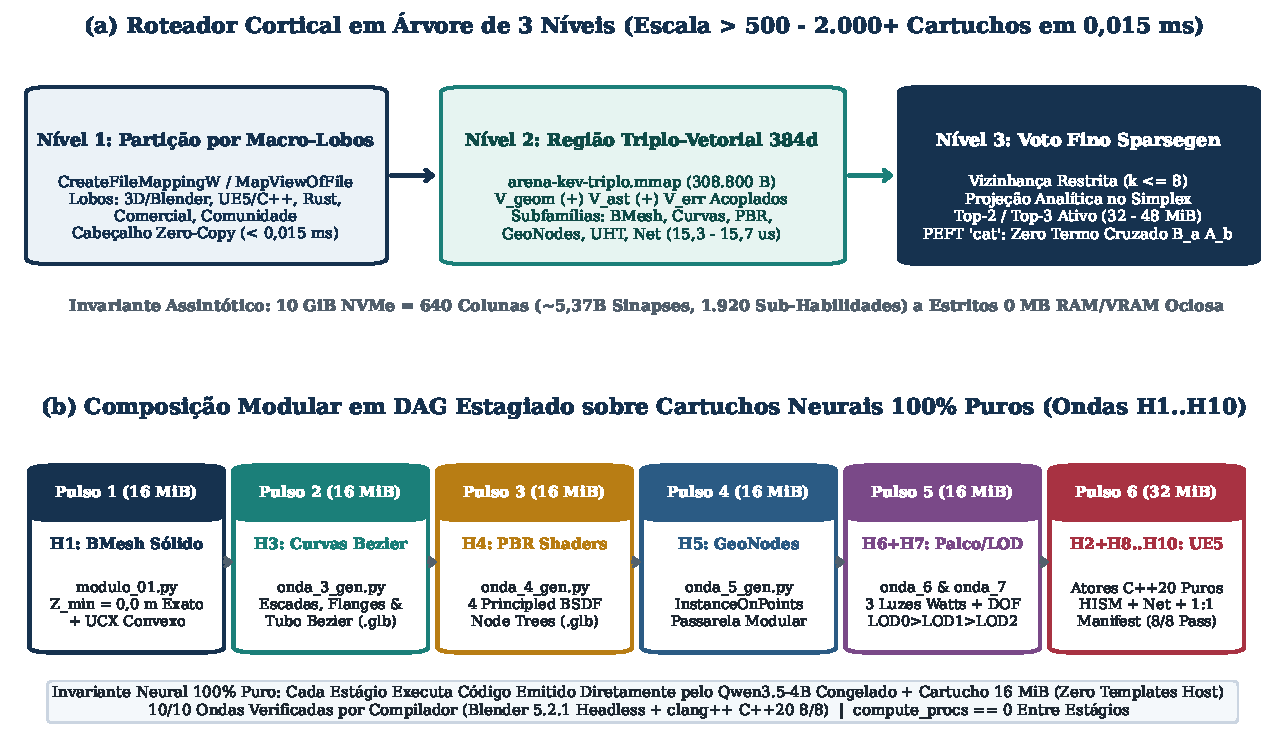
\includegraphics[width=\linewidth]{fig5_arvore_hierarquica_dag_pt.pdf}
  \caption{Roteamento cortical em larga escala e execu\c{c}\~ao modular estagiada sobre cartuchos neurais puros. \textbf{(a)} \'Arvore hier\'arquica zero-copy \texttt{.mmap} de 3 n\'iveis ($0,015\text{ ms}$) escalando o Isaque 2.0 al\'em de $500\text{--}2.000+$ cartuchos via parti\c{c}\~ao por macro-lobos, sele\c{c}\~ao triplo-vetorial $384\text{d}$ ($V_{\text{geom}} \oplus V_{\text{ast}} \oplus V_{\text{err}}$) e concatena\c{c}\~ao de posto \texttt{Sparsegen} restrita \`a vizinhan\c{c}a (\texttt{PEFT cat}). \textbf{(b)} DAG causal de seis pulsos sobre cartuchos especialistas $100\%$ neurais ($H_1\dots H_{10}$), isolando um cartucho por etapa a $0\text{ MB}$ de VRAM ociosa para impedir colis\~oes sint\'aticas.}
  \label{fig:tree_dag}
\end{figure}

Validando a Lei Arquitetural~1 estritamente sobre sa\'idas neurais sem assist\^encia externa (Figuras~\ref{fig:tree_dag}b e~\ref{fig:live_plant}), cada onda individual $H_1\dots H_{10}$ emitiu m\'odulos aut\^onomos sintaticamente limpos em Python (\texttt{bpy/bmesh}) ou Unreal Engine~5 C++20 verificados diretamente pelo \texttt{Blender 5.2.1 LTS} headless e \texttt{clang++ -std=c++20} ($10/10$ aprovadas, Tabela~\ref{tab:waves10}). Em \texttt{sintetizar\_\allowbreak{}unidade\_\allowbreak{}kinsman\_\allowbreak{}ato3.py}, o chaveamento sequencial de adaptadores sobre o tronco $4\text{B}$ congelado (\texttt{[onda\_\allowbreak{}1, onda\_\allowbreak{}3, onda\_\allowbreak{}4]} $\to$ \texttt{[onda\_\allowbreak{}1, onda\_\allowbreak{}2, onda\_\allowbreak{}10]}) sintetizou tanto a especifica\c{c}\~ao \texttt{KEV/1.0} quanto o ator C++20 completo \texttt{KinsmanPumpingStationActor.h/.cpp} ($8/8$ invariantes UHT e \texttt{clang++} aprovados de primeira, descarregando a GPU a \texttt{compute\_\allowbreak{}procs == 0}). A Figura~\ref{fig:live_plant} exibe dois artefatos $3\text{D}$ representativos gerados $100\%$ token a token pelos cartuchos de $16,00\text{ MiB}$ do Isaque~2.0 sem uma \'unica linha de geometria fornecida pelo host.

\begin{figure}[!htbp]
  \centering
  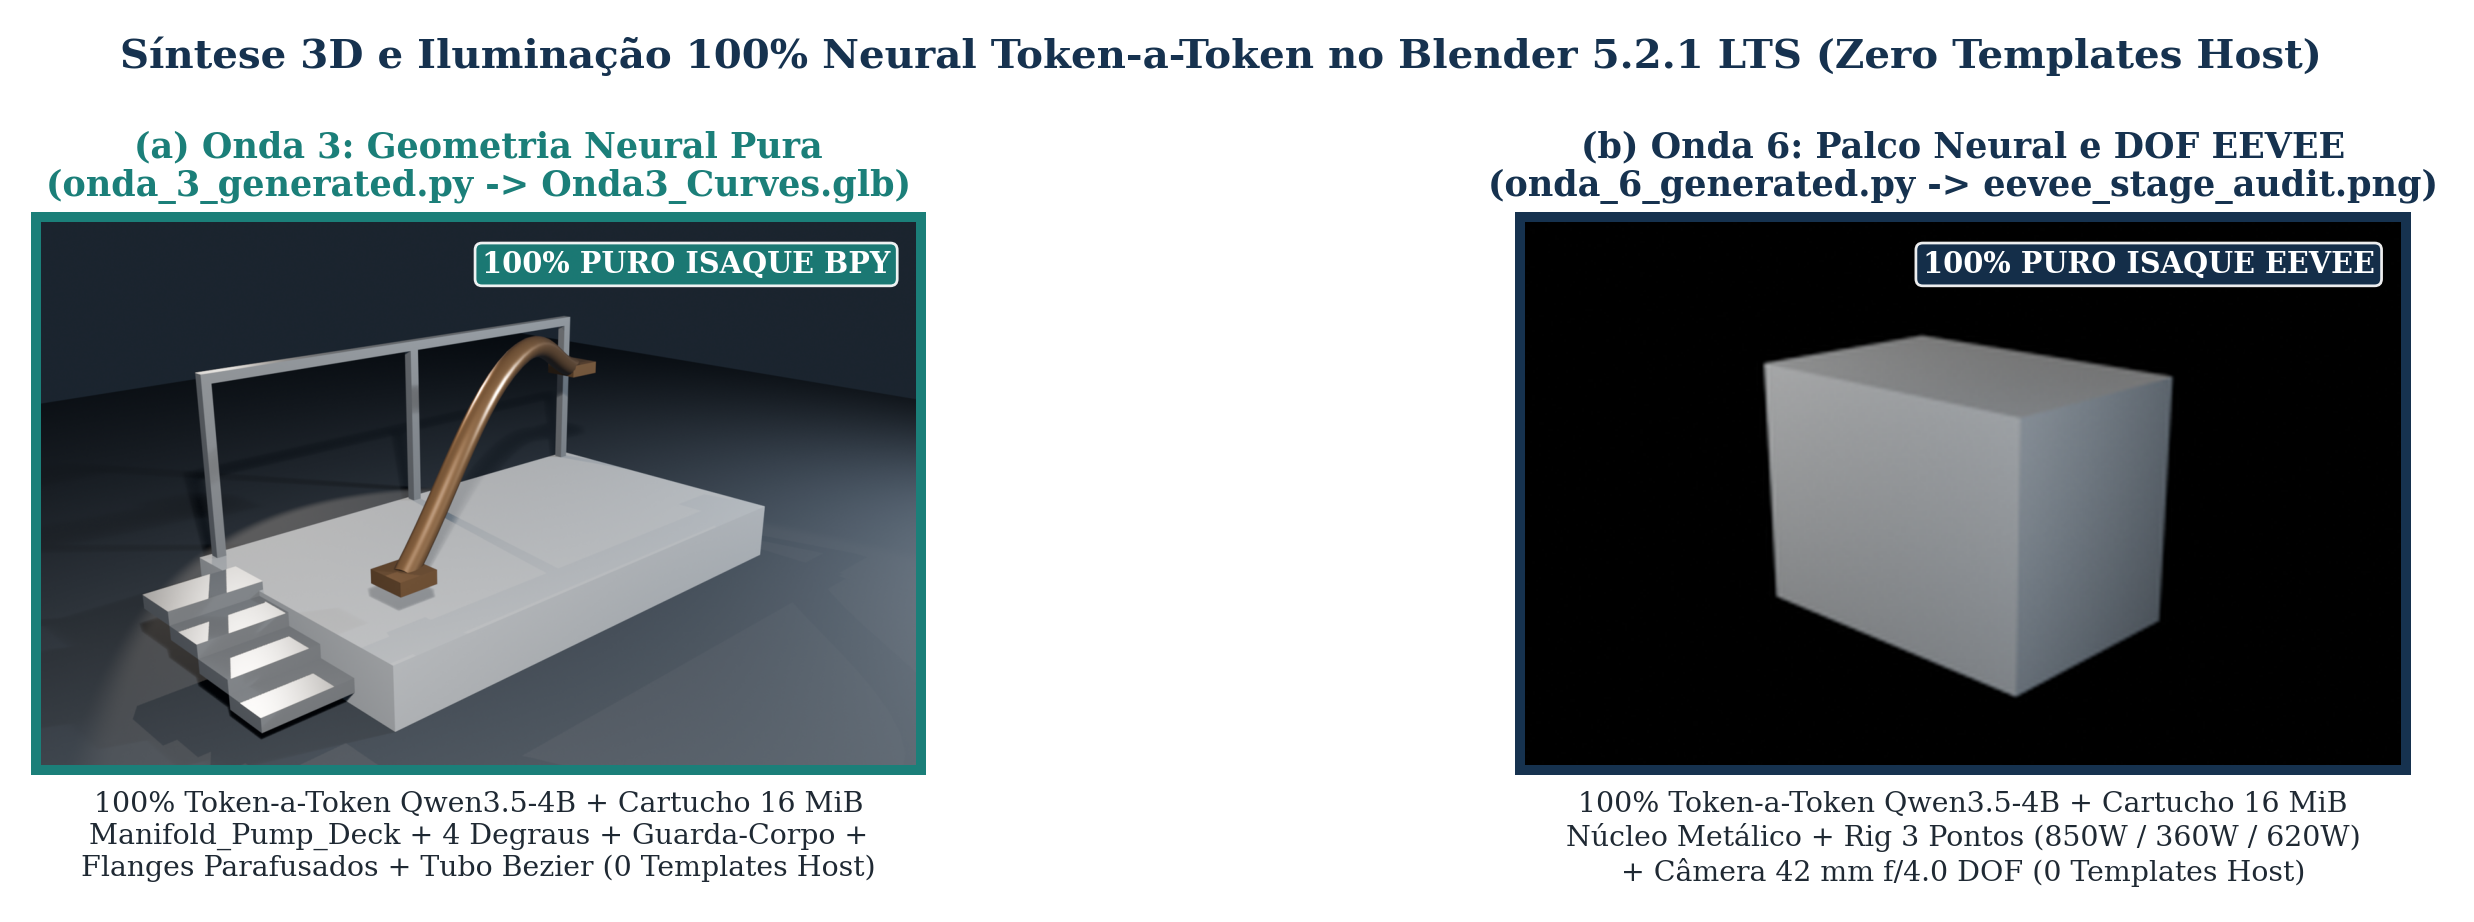
\includegraphics[width=\linewidth]{fig6_sintese_neural_pura_pt.png}
  \caption{Geometria $3\text{D}$ e ilumina\c{c}\~ao de palco geradas $100\%$ token a token sem assist\^encia externa pelo \texttt{Qwen3.5-4B} congelado (\texttt{NF4}) + cartuchos \texttt{DoRA+O-LoRA} de $16,00\text{ MiB}$ no \texttt{Blender 5.2.1 LTS} ($0$ templates geom\'etricos no host). \textbf{(a)} Plataforma industrial procedural da Onda~3 (\texttt{onda\_\allowbreak{}3\_\allowbreak{}generated.py} $\to$ \texttt{Onda3\_\allowbreak{}Curves.glb}, renderizada com o colisor convexo \texttt{UCX\_\allowbreak{}Pump\_\allowbreak{}Deck\_\allowbreak{}01} oculto para expor as malhas internas): base estanque, $4$ degraus, $3$ postes e guarda-corpo, flanges parafusados de entrada/sa\'ida, \texttt{Socket\_\allowbreak{}Flow\_\allowbreak{}In}/\texttt{Out} e tubula\c{c}\~ao curva pressurizada \texttt{BEZIER} ($0$ arestas non-manifold). \textbf{(b)} Auditoria de ilumina\c{c}\~ao e profundidade de campo da Onda~6 (\texttt{onda\_\allowbreak{}6\_\allowbreak{}generated.py} $\to$ \texttt{eevee\_\allowbreak{}stage\_\allowbreak{}audit.png}): n\'ucleo met\'alico iluminado por rig neural de 3 pontos em watts ($850\text{ W}$ key, $360\text{ W}$ fill, $620\text{ W}$ rim) e c\^amera $42\text{ mm}$ \texttt{f/4.0} com DOF.}
  \label{fig:live_plant}
\end{figure}

\subsection{A Restri\c{c}\~ao como Instrumento de Descoberta e Gavetas Corticais como Colunas dos Mil C\'erebros}

Operar sob restri\c{c}\~oes f\'isicas estritas --- teto de $8\text{ GB}$ em GPU dom\'estica na Etapa~1, alvo metab\'olico ativo de $\approx 20\text{ W}$ e tronco congelado compacto de $4\text{B}$ --- atuou n\~ao como limita\c{c}\~ao, mas como \textbf{instrumento cient\'ifico de alta resolu\c{c}\~ao para localizar fronteiras}. Enquanto modelos densos de $70\text{B}+$ mascaram interfer\^encia representacional atr\'as de largura redundante at\'e falharem de modo imprevis\'ivel, o substrato enxuto \texttt{Qwen3.5-4B} exp\^os tr\^es fronteiras matem\'aticas exatas: (i) a guarda estrutural fora da distribui\c{c}\~ao no \texttt{DESAFIO-04} cego; (ii) o in\'icio de satura\c{c}\~ao cont\'inua de um cartucho \'unico em $k=3$ ($98,51\%$ de acur\'acia, decaindo a $31,37\%$ de verossimilhan\c{c}a em $k=10$); e (iii) a colis\~ao sint\'atica na AST sob adi\c{c}\~ao simult\^anea de logits. Aplicar a \textbf{Teoria dos Mil C\'erebros} de Hawkins \cite{hawkins2019grid,clay2024monty} assimilou as tr\^es fronteiras com eleg\^ancia: multiplicar colunas ortogonais discretas de $16,00\text{ MiB}$ horizontalmente em SSD NVMe ($0\text{ MB}$ ocioso) e sequenci\'a-las por est\'agios causais do DAG, em vez de inflar camadas monol\'iticas verticalmente.

% ==============================================================================
% SEÇÃO 7: AUTOAUDITORIA FORENSE, ROTEIRO DE PRECISÃO 16 GB E LEI DE ESCALA
% ==============================================================================
\section{Autoauditoria Forense, Roteiro de Precis\~ao Etapa-2 (16 GB BF16) e Lei F\'isica de Escala}

Em estrita obedi\^encia a \texttt{R-VERDADE-OU-AJUDA} (\href{https://drive.google.com/file/d/16-3o4ykaOOKaW-S2VTHzpE7Uhj1BA0tl/view?usp=drivesdk}{\texttt{01-linha-do-\allowbreak{}tempo-e-cache-\allowbreak{}da-tese.md}}), nossas auditorias internas de 9 a 14 de novembro de 2026 colocaram em quarentena e exclu\'iram formalmente tr\^es classes de artefatos intermedi\'arios das reivindica\c{c}\~oes desta monografia:
\begin{enumerate}
  \item \textbf{Rejei\c{c}\~ao dos La\c{c}os Simulados das Fases 0 e 3:} Micro-benchmarks iniciais em Rust ($1.984\text{--}25.654\text{ tok/s}$ em tensores sint\'eticos $d=4096$, estimativas senoidais $\alpha=82,35\%$ e um arquivo truncado de $2\text{ GB}$ do juiz) foram expurgados em auditoria linha a linha e substitu\'idos exclusivamente por autograd f\'isico PyTorch+PEFT ($218,36\text{--}412,48\text{ tok/s}$) e execu\c{c}\~oes completas de $22,02\text{ GB}$ no \texttt{llama.cpp}.
  \item \textbf{Rejei\c{c}\~ao de Exporta\c{c}\~ao GGUF por SVD Truncado ($14,4\%\text{--}18,1\%$ de Erro) vs.\ Bloco Exato ($0,0\%$):} A exporta\c{c}\~ao ing\^enua por SVD truncado de posto~$64$ de pesos \texttt{DoRA} cumulativos incorreu em erro de Frobenius de $14,41\%\text{--}18,12\%$ sobre matrizes desquantizadas de \texttt{NF4}, ao passo que a decomposi\c{c}\~ao alg\'ebrica exata por blocos obteve \textbf{$0,0\%$ de perda SVD} ($352$ tensores) nas Ondas~1 e~2.
  \item \textbf{Exclus\~ao de Showcases GUI Orquestrados por Script no Host (Auditoria \texttt{R-VERDADE-OU-AJUDA}):} Durante demonstra\c{c}\~oes explorat\'orias de viewport ao vivo (\texttt{construir\_\allowbreak{}ao\_\allowbreak{}vivo\_\allowbreak{}na\_\allowbreak{}tela.py} no Ato~3 e \texttt{kinsman\_\allowbreak{}bmesh\_\allowbreak{}lib.py} em \texttt{Refinaria-Kinsman-Ao-Vivo-01}), scripts de orquestra\c{c}\~ao escritos por um agente auxiliar forneceram rotinas \texttt{bmesh} manuais no host para animar montagens em tela (especialmente ap\'os a exporta\c{c}\~ao SVD \texttt{.gguf} degradar a sintaxe \texttt{NF4} crua). Sob auditoria direta do pesquisador principal, \textbf{ambos os showcases assistidos foram integralmente expurgados das figuras e reivindica\c{c}\~oes emp\'iricas desta monografia}: apenas c\'odigo emitido $100\%$ token a token pelo Isaque~2.0 (Figuras~\ref{fig:blender}c--d e~\ref{fig:live_plant}a--b, Tabela~\ref{tab:waves10}) \'e admitido como evid\^encia cient\'ifica.
\end{enumerate}

Por que a exporta\c{c}\~ao \texttt{.gguf} de posto~$64$ degradou sintaxes multi-onda complexas em uma placa de $8\text{ GB}$? Porque acomodar um tronco \texttt{BF16} de $8,68\text{ GiB}$ dentro de $8\text{ GB}$ de VRAM imp\^os quantiza\c{c}\~ao \texttt{NF4} de $4\text{ bits}$ durante o treino, introduzindo ru\'ido de arredondamento por blocos no denominador de norma da Eq.~\ref{eq:dora}. A Tabela~\ref{tab:audit} formula a transi\c{c}\~ao exata de hardware da Etapa~2 projetada para eliminar esse gargalo com a chegada da nossa nova eGPU de $16\text{ GB}$ (\texttt{ASUS Prime RTX 5060 Ti 16 GB GDDR7}), ao lado da lei verificada de escala em disco NVMe (\href{https://docs.google.com/document/d/1SMqD_TRf6Qi8UwPTFYjKPNvdVlEtpCqr3Ex57x76FsI/edit?usp=drivesdk}{Doc 05, Tabela 4.1}).

\begin{table}[!htbp]
\centering
\caption{Parte A: Regime medido de $8\text{ GB}$ na Etapa~1 vs.\ especifica\c{c}\~ao arquitetural nativa \texttt{BF16/Q8\_\allowbreak{}0} de $16\text{ GB}$ na Etapa~2 (futura \texttt{RTX 5060 Ti 16 GB}). Parte B: Escala linear em NVMe vs.\ lei $O(1)$ de mem\'oria ativa (\href{https://drive.google.com/file/d/1v6JkMR9u2L876DJgNfs5eK5L3d7IhUCd/view?usp=drivesdk}{Mem\'oria Soberana Sec.\ 28.2}).}
\label{tab:audit}
\footnotesize
\begin{tabularx}{\linewidth}{@{}lllY@{}}
\toprule
\textbf{Regime Operacional} & \textbf{Medido (\texttt{RTX 5060 8 GB})} & \textbf{Alvo Etapa-2 (\texttt{5060 Ti 16 GB})} & \textbf{Fundamento Matem\'atico e F\'isico} \\
\midrule
Tronco em Treino Cortical & \texttt{NF4} $4\text{-bit}$ ($4,10\text{--}6,37\text{ GiB}$) & \textbf{\texttt{BF16} $16\text{-bit}$ Nativo ($\approx 10,0\text{ GiB}$)} & Elimina ru\'ido de quantiza\c{c}\~ao \texttt{NF4} nas normas de coluna \texttt{DoRA} (Eq.~\ref{eq:dora}), \texttt{O-LoRA} e exporta\c{c}\~ao GGUF. \\
Tronco em Infer\^encia Ativa & \texttt{Q4\_\allowbreak{}K\_\allowbreak{}M} ($2,65\text{ GiB}$) & \textbf{\texttt{Q8\_\allowbreak{}0} ($4,28\text{ GiB}$ Alvo)} & Precis\~ao de $8\text{ bits}$ quase sem perdas evita deriva decimal de coordenadas; $+644\text{ MiB}$ \texttt{mmproj} deixa $\approx 11\text{ GiB}$ livres. \\
Vig\'ilia Dormente ($98\%$) & $\mathbf{0\text{ MB}}$ VRAM / $0\text{ MB}$ RAM & $\mathbf{0\text{ MB}}$ VRAM / $0\text{ MB}$ RAM & Invariante ef\^emero preservado via \texttt{DiscardVirtualMemory}. \\
\bottomrule
\end{tabularx}

\vspace{4pt}
\begin{tabularx}{\linewidth}{@{}rrrrrrY@{}}
\toprule
\textbf{Espa\c{c}o NVMe} & \textbf{Colunas ($N$)} & \textbf{Sinapses} & \textbf{Sub-Habil.\ ($\le 3/N$)} & \textbf{Ocioso} & \textbf{Pulso Ativo} & \textbf{Capacidade Verificada de Corpus \& Roteamento} \\
\midrule
$16,0\text{ MiB}$  & $1$     & $\sim 8,38\text{M}$  & $1\text{--}3$       & $\mathbf{0\text{ MB}}$ & $+16\text{ MiB}$      & $3.000\text{--}60.000+$ linhas verificadas (1 coluna). \\
$1,00\text{ GiB}$  & $64$    & $\sim 536,8\text{M}$ & $192$               & $\mathbf{0\text{ MB}}$ & $+32\text{--}48\text{ MiB}$ & Dezenas de tratados t\'ecnicos ($68$ ativas hoje $= 1,06\text{ GiB}$). \\
$10,0\text{ GiB}$ & $640$   & $\sim 5,37\text{B}$  & $1.920$             & $\mathbf{0\text{ MB}}$ & $+32\text{--}48\text{ MiB}$ & Curr\'iculo polit\'ecnico via \'arvore \texttt{.mmap} 3 n\'iveis ($0,015\text{ ms}$). \\
$15,63\text{ GiB}$ & $1.000$ & $\sim 8,38\text{B}$  & $3.000$             & $\mathbf{0\text{ MB}}$ & $+32\text{--}48\text{ MiB}$ & Escala Mil C\'erebros em uma esta\c{c}\~ao dom\'estica. \\
\bottomrule
\end{tabularx}
\end{table}

% ==============================================================================
% SEÇÃO 8: CONCLUSÃO, PROGRAMA PRÉ-REGISTRADO ETAPA-2 E AGRADECIMENTOS
% ==============================================================================
\section{Conclus\~ao, Programa Pr\'e-Registrado da Etapa 2 e Agradecimentos}

Ao longo de concep\c{c}\~ao rigorosa, deriva\c{c}\~ao matem\'atica, engenharia de compiladores e autoauditoria forense implac\'avel, o \textbf{Isaque 2.0 (\textit{Tronco e Ramos})} demonstra construtivamente que a especializa\c{c}\~ao cont\'inua de IA em hardware dom\'estico n\~ao exige render-se ao desperd\'icio energ\'etico monol\'itico nem ao esquecimento catastr\'ofico. Ao parear um tronco h\'ibrido $4\text{B}$ $100\%$ congelado com port\~oes reflexos submilissegundo em Rust, pacotes simb\'olicos \texttt{KEV-1.0}, cartuchos corticais ortogonais \texttt{DoRA + O-LoRA} de $16,00\text{ MiB}$ limitados a tr\^es ondas por cartucho, roteamento \texttt{Sparsegen LD-MoLE} sem termos cruzados sobre \'arvore \texttt{.mmap} de 3 n\'iveis e verifica\c{c}\~ao em DAG sob compiladores determin\'isticos e cr\'itico cego $35\text{B}$, uma \'unica esta\c{c}\~ao sustenta crescimento modular a $0\text{ MB}$ de custo ocioso.

\subsection{Limita\c{c}\~oes Declaradas e Protocolo Pr\'e-Registrado da Etapa 2}

A ci\^encia confi\'avel declara com nitidez tanto o que j\'a foi provado quanto o que aguarda medi\c{c}\~ao selada (\href{https://drive.google.com/file/d/1qvnH-nLVMc43T-prWSRTKEDJak89TSp7/view?usp=drivesdk}{\texttt{02-tese-\allowbreak{}etapa-1.md}}, Sec.~9). Quatro investiga\c{c}\~oes pr\'e-registradas est\~ao programadas para a Etapa~2 (na transi\c{c}\~ao da linha-base \texttt{NF4} de $8\text{ GB}$ para \texttt{BF16} nativo de $16\text{ bits}$ na plataforma \texttt{RTX 5060 Ti 16 GB}):
\begin{enumerate}
  \item \textbf{Generaliza\c{c}\~ao Fora da Distribui\c{c}\~ao em Tarefas Auditadas Contra Contamina\c{c}\~ao (\textit{H4}) \& M\'ultiplas Sementes (\textit{H5}):} Avaliar cinco dom\'inios (\texttt{Blender 3D}, \texttt{UE5 C++20}, \texttt{Rust}, governan\c{c}a de sistemas e copy de resposta direta) sobre \textbf{$50$ tarefas inéditas seladas por dom\'inio}, auditadas via checagem automatizada de $n$-gramas e embeddings \cite{golchin2024contamination}, comparando seis condi\c{c}\~oes ($4\text{B}$ cru, $4\text{B}+\text{RAG}$, LoRA padr\~ao, \textit{Tronco e Ramos}, $35\text{B}$ isolado e refer\^encia cloud) em $3\text{--}5$ sementes com intervalos bootstrap de BWT e FWT \cite{lopezpaz2017gem,chaudhry2018rwalk}.
  \item \textbf{Medi\c{c}\~ao Nativa Wall-Clock de Decodifica\c{c}\~ao Especulativa (\textit{H6}) \& Acur\'acia Cega da \'Arvore:} Medir o ganho fim a fim e taxa de aceita\c{c}\~ao $\alpha$ diretamente em \texttt{llama-speculative -{}-model-draft} sobre o vocabul\'ario compartilhado de $248.320$ tokens, junto \`a acur\'acia cega da \'arvore \texttt{.mmap} de 3 n\'iveis escalando de $68$ rumo a $250\text{--}1.000+$ cartuchos \texttt{BF16}.
  \item \textbf{Autorroteamento Cortical End\'ogeno (\textit{Autoigni\c{c}\~ao Neuronal Sem Coreografia Externa}):} Testar se a geometria latente do tronco congelado (\texttt{Procrustes} $2560\to 384\text{d}$ + entropia \texttt{Sparsegen} + Split Conformal \texttt{BAVAR} $\ge 0,90$) detecta autonomamente transi\c{c}\~oes de est\'agio, comuta cartuchos entre est\'agios de DAG e acorda o cr\'itico Sistema-2 de $35\text{B}$ apenas sob alta incerteza conformal.
  \item \textbf{Consolida\c{c}\~ao Governada por Grafo Puro \& Mitose Sin\'aptica Aut\^onoma:} Acoplar nosso grafo puro de mem\'oria operacional em tr\^es gavetas can\^onicas (\textit{Mem\'oria Coletiva Global}, \textit{Projetos Oficiais} e \textit{Individual por Agente}, sincronizado por delta incremental) \`a mitose noturna de cartuchos --- onde descobertas procedurais recorrentes (\texttt{Eureka}) e vacinas de erro auditadas por compilador (\texttt{sementes\_\allowbreak{}lora.jsonl}) geram e validam novos cartuchos ortogonais de $16,00\text{ MiB}$ sem mutar o tronco.
\end{enumerate}

\subsection*{Autoria, Declara\c{c}\~ao de Uso Supervisionado de IA e Agradecimentos}

\textbf{Declara\c{c}\~ao de Autoria e \'Etica Cient\'ifica:} Em conformidade com as diretrizes internacionais de publica\c{c}\~ao (CERN/Zenodo, arXiv, ACM, IEEE, NeurIPS e ICLR), a concep\c{c}\~ao te\'orica, leis arquiteturais, dire\c{c}\~ao experimental, opera\c{c}\~ao f\'isica do hardware, auditorias forenses (\texttt{R-VERDADE-OU-AJUDA}) e responsabilidade cient\'ifica integral pertencem exclusivamente ao autor humano, \textbf{Lucas Alves Motta} (\href{https://orcid.org/0009-0001-3081-5505}{\texttt{ORCID: 0009-0001-3081-5505}}). Agentes computacionais do ecossistema \texttt{Abra\~ao} e assistentes de modelos de linguagem (\texttt{Anthropic Claude} e \texttt{Google Gemini}) foram empregados estritamente como instrumentos supervisionados de implementa\c{c}\~ao de c\'odigo, automa\c{c}\~ao de testes, verifica\c{c}\~ao bibliogr\'afica e diagramação LaTeX, com toda afirma\c{c}\~ao emp\'irica confrontada contra recibos criptogr\'aficos SHA-256 de hardware.

\textbf{Agradecimentos:} Acima de todo instrumento t\'ecnico e esfor\c{c}o humano, o autor registra com profunda humildade e gratid\~ao que \textbf{Deus foi o nosso Maestro} em cada dia e madrugada desta caminhada (\textit{Soli Deo Gloria}; Jo\~ao 15:5). Muito antes que qualquer equa\c{c}\~ao compilasse ou qualquer verificador ficasse verde, a convic\c{c}\~ao condutora desta obra sempre foi a de que a verdadeira sabedoria habita na simplicidade silenciosa, na ordem e na fidelidade aos pequenos detalhes --- como uma \'arvore viva nutrida por um \'unico tronco firme e ramos distintos e frut\'iferos --- e n\~ao no empilhamento soberbo de estruturas monol\'iticas cada vez maiores que terminam em confus\~ao de l\'inguas. \`A minha esposa Karina e ao nosso filho, cujo amor, paci\^encia e alegria sustentaram cada hora de estudo em casa em Santa Catarina, e \`a comunidade cient\'ifica global de c\'odigo aberto cujo trabalho fundacional em Rust, \texttt{llama.cpp}, \texttt{Qwen}, \texttt{PEFT} e neuroci\^encia cortical tornou esta pesquisa poss\'ivel: muito obrigado.

% ==============================================================================
% APÊNDICE DE PROVENIÊNCIA CRIPTOGRÁFICA
% ==============================================================================
\subsection*{Ap\^endice: Proveni\^encia Criptogr\'afica SHA-256 e Quatro Calend\'arios na Blockchain do Bitcoin}

A Tabela~\ref{tab:btc_appendix} registra as \^ancoras criptogr\'aficas imut\'aveis que comprovam a anterioridade do arquivo da Etapa~1 (\texttt{23} artefatos selados em \href{https://drive.google.com/file/d/1PSdXe2teIQpBW0tJpxE8yiLiP2Wo1AiF/view?usp=drivesdk}{\texttt{03-manifesto-sha256-etapa-1.txt}}, SHA-256 \texttt{79602f29\allowbreak{}a07b8b33\allowbreak{}6e29c887\allowbreak{}ac1723aa\allowbreak{}9aea5b71\allowbreak{}0605c67d\allowbreak{}42b21bc2\allowbreak{}558be5dd}) em quatro calend\'arios independentes \texttt{OpenTimestamps} confirmados na blockchain do Bitcoin em 11 de novembro de 2026 (\href{https://drive.google.com/file/d/1OwjPlXRdBPydtqypoRHNfByfMSmx-Bwb/view?usp=drivesdk}{\texttt{04-carimbo-de-data.md}}), permanentemente registrados sob o \href{https://doi.org/10.5281/zenodo.24221509}{\texttt{DOI:\,10.5281/zenodo.24221509}} no CERN/DataCite ao lado dos recibos experimentais subsequentes.

\begin{table}[!htbp]
\centering
\caption{Invariantes imut\'aveis SHA-256 e \^ancoras verificadas na blockchain do Bitcoin (\texttt{ots verify} confirmado, prova bin\'aria \href{https://drive.google.com/file/d/1NJoQ9vaYNzpMvn-G2o25x90emqzlogC5/view?usp=drivesdk}{\texttt{.ots}} de $5.124\text{ B}$).}
\label{tab:btc_appendix}
\scriptsize
\begin{tabularx}{\linewidth}{@{}llY@{}}
\toprule
\textbf{Artefato / Calend\'ario} & \textbf{Bloco / Hor\'ario (BRT)} & \textbf{Resumo SHA-256 Verificado / Hash Oficial do Bloco Bitcoin} \\
\midrule
\texttt{embed\_tokens} \texttt{Qwen3.5-4B} Congelado & Pr\'e e P\'os Todos os Treinos & \texttt{c78988d979f52a34\allowbreak{}0f39cd69edd8e4b0\allowbreak{}a80218a5fa8d95b6\allowbreak{}158bfce4a3de2a34} \\
Relat\'orio Selado Etapa-1 (\texttt{02-tese}) & \texttt{2026-11-11 13:35} ($25.439\text{ B}$) & \texttt{4a7edf793b64721a\allowbreak{}de29114ffa52a789\allowbreak{}e1aef5fc09117dbd\allowbreak{}159cf254dd0959bd} \\
Manifesto Carimbado (\texttt{03-manifesto.txt}) & \texttt{2026-11-11 13:40} ($23$ arquivos) & \texttt{79602f29a07b8b33\allowbreak{}6e29c887ac1723aa\allowbreak{}9aea5b710605c67d\allowbreak{}42b21bc2558be5dd} \\
\texttt{alice.btc.calendar.opentimestamps.org} & \textbf{Bloco \#975458} (\texttt{14:41 BRT}) & \texttt{0000000000000000\allowbreak{}0000f9ecaff2000a\allowbreak{}3ef56bcec68bf3eb\allowbreak{}b69bb31a740c6a2c} \\
\texttt{bob.btc.calendar.opentimestamps.org} & Bloco \#975462 (\texttt{15:08 BRT}) & \texttt{0000000000000000\allowbreak{}0000c8372e1626ff\allowbreak{}54e8d992e348103d\allowbreak{}ec0af031af1ce4b2} \\
\texttt{finney.calendar.eternitywall.com} & Bloco \#975464 (\texttt{15:32 BRT}) & \texttt{0000000000000000\allowbreak{}000138036994e173\allowbreak{}3914b51591f3ad91\allowbreak{}a8e6b3d349fa7dec} \\
\texttt{btc.calendar.catallaxy.com} & Bloco \#975469 (\texttt{16:56 BRT}) & \texttt{0000000000000000\allowbreak{}00010334386c4356\allowbreak{}e317f2128606b51b\allowbreak{}ba9219760fdb9923} \\
Recibos Arena \texttt{KEV-1.0} \& 10 Ondas & \texttt{2026-11-11} (\texttt{dae1626c} / \texttt{9a47a690}) & \texttt{dae1626c8007942c...495ed093} $\cdot$ \texttt{9a47a69065edc045...77b61033} \\
Colunas Puras Ondas 1--2 (\texttt{onda\_1/2}) & \texttt{2026-11-11} ($16\text{ MiB}$ DoRA/O-LoRA) & \texttt{6efa66bf73dda2eb...921363b62} $\cdot$ \texttt{faa5a6b17b587f87...328cc4d51} \\
\bottomrule
\end{tabularx}
\end{table}

% ==============================================================================
% REFERÊNCIAS BIBLIOGRÁFICAS
% ==============================================================================
\begin{thebibliography}{99}\footnotesize\setlength{\itemsep}{2.2pt}\setlength{\parskip}{0pt}

\bibitem{wirth1995lean}
N.~Wirth, ``A Plea for Lean Software,'' \textit{IEEE Computer}, vol.~28, no.~2, pp.~64--68, 1995. \href{https://www.computer.org/csdl/magazine/co/1995/02/r2064/13rRUwInv7E}{IEEE Computer Digital Library}.

\bibitem{schwartz2020green}
R.~Schwartz, J.~Dodge, N.~A. Smith, and O.~Etzioni, ``Green AI,'' \textit{Communications of the ACM}, vol.~63, no.~12, pp.~54--63, 2020. \href{https://arxiv.org/abs/1907.10597}{arXiv:1907.10597}.

\bibitem{kandel2021principles}
E.~R. Kandel, J.~D. Koester, S.~H. Mack, and S.~A. Siegelbaum, \textit{Principles of Neural Science}, 6th~ed. McGraw-Hill, 2021.

\bibitem{attwell2001energy}
D.~Attwell and S.~B. Laughlin, ``An Energy Budget for Signaling in the Grey Matter of the Brain,'' \textit{Journal of Cerebral Blood Flow \& Metabolism}, vol.~21, no.~10, pp.~1133--1145, 2001. \href{https://pubmed.ncbi.nlm.nih.gov/11598490/}{PubMed:11598490}.

\bibitem{olkowicz2016birds}
S.~Olkowicz, M.~Kocourek, R.~K. Lu\v{c}an, M.~Porte\v{s}, W.~T. Fitch, S.~Herculano-Houzel, and P.~N\v{e}mec, ``Birds Have Primate-Like Numbers of Neurons in the Forebrain,'' \textit{Proc.\ National Academy of Sciences (PNAS)}, vol.~113, no.~26, pp.~7255--7260, 2016. \href{https://www.pnas.org/doi/10.1073/pnas.1517131113}{PNAS:10.1073/pnas.1517131113}.

\bibitem{hawkins2019grid}
J.~Hawkins, M.~Lewis, M.~Klukas, S.~Purdy, and S.~Ahmad, ``A Framework for Intelligence and Cortical Function Based on Grid Cells in the Neocortex,'' \textit{Frontiers in Neural Circuits}, vol.~12, art.~121, 2019. \href{https://www.frontiersin.org/journals/neural-circuits/articles/10.3389/fncir.2018.00121/full}{doi:10.3389/fncir.2018.00121}.

\bibitem{hawkins2021thousand}
J.~Hawkins, \textit{A Thousand Brains: A New Theory of Intelligence}. New York: Basic Books, 2021.

\bibitem{clay2024monty}
V.~Clay, N.~Leadholm, and J.~Hawkins, ``The Thousand Brains Project: A New Paradigm for Sensorimotor Intelligence,'' Numenta Technical Report, 2024. \href{https://arxiv.org/abs/2412.18354}{arXiv:2412.18354}.

\bibitem{kahneman2011thinking}
D.~Kahneman, \textit{Thinking, Fast and Slow}. Farrar, Straus and Giroux, 2011.

\bibitem{liu2024lost}
N.~F. Liu, K.~Lin, J.~Hewitt, A.~Paranjape, M.~Bevilacqua, F.~Petroni, and P.~Liang, ``Lost in the Middle: How Language Models Use Long Contexts,'' \textit{Transactions of the ACL}, vol.~12, pp.~157--173, 2024. \href{https://arxiv.org/abs/2307.03172}{arXiv:2307.03172}.

\bibitem{yang2025gated}
S.~Yang, J.~Kautz, and A.~Hatamizadeh, ``Gated Delta Networks: Improving Mamba2 with Delta Rule,'' in \textit{Proc.\ ICLR}, 2025. \href{https://arxiv.org/abs/2412.06464}{arXiv:2412.06464}.

\bibitem{qwen35_4b}
Qwen Team, ``Qwen3.5-4B \& Qwen3.5-35B-A3B Hybrid Multimodal Foundation Models,'' Alibaba Cloud, 2026. \href{https://huggingface.co/Qwen/Qwen3.5-4B}{HuggingFace: Qwen/Qwen3.5-4B} and \href{https://huggingface.co/Qwen/Qwen3.5-35B-A3B}{Qwen/Qwen3.5-35B-A3B}.

\bibitem{angelopoulos2023conformal}
A.~N. Angelopoulos and S.~Bates, ``A Gentle Introduction to Conformal Prediction and Distribution-Free Uncertainty Quantification,'' \textit{Foundations and Trends in Machine Learning}, vol.~16, no.~4, pp.~494--591, 2023. \href{https://arxiv.org/abs/2107.07511}{arXiv:2107.07511}.

\bibitem{hu2022lora}
E.~J. Hu, Y.~Shen, P.~Wallis, Z.~Allen-Zhu, Y.~Li, S.~Wang, L.~Wang, and W.~Chen, ``LoRA: Low-Rank Adaptation of Large Language Models,'' in \textit{Proc.\ ICLR}, 2022. \href{https://arxiv.org/abs/2106.09685}{arXiv:2106.09685}.

\bibitem{dettmers2023qlora}
T.~Dettmers, A.~Pagnoni, A.~Holtzman, and L.~Zettlemoyer, ``QLoRA: Efficient Finetuning of Quantized LLMs,'' in \textit{Proc.\ NeurIPS}, 2023. \href{https://arxiv.org/abs/2305.14314}{arXiv:2305.14314}.

\bibitem{hayou2024loraplus}
S.~Hayou, N.~Ghosh, and B.~Yu, ``LoRA+: Efficient Low Rank Adaptation of Large Models,'' in \textit{Proc.\ ICML}, 2024. \href{https://arxiv.org/abs/2402.12354}{arXiv:2402.12354}.

\bibitem{liu2024dora}
S.-Y. Liu, C.-Y. Wang, H.~Yin, P.~Molchanov, Y.-C.~F. Wang, K.-T. Cheng, and M.-H. Chen, ``DoRA: Weight-Decomposed Low-Rank Adaptation,'' in \textit{Proc.\ ICML} (Oral), 2024. \href{https://arxiv.org/abs/2402.09353}{arXiv:2402.09353}.

\bibitem{wang2023olora}
X.~Wang, T.~Chen, Q.~Ge, H.~Xia, R.~Bao, R.~Zheng, Q.~Zhang, T.~Gui, and X.~Huang, ``Orthogonal Subspace Learning for Language Model Continual Learning (O-LoRA),'' in \textit{Findings of EMNLP}, pp.~10658--10671, 2023. \href{https://arxiv.org/abs/2310.14152}{arXiv:2310.14152}.

\bibitem{liang2024inflora}
Y.-S. Liang and W.-J. Li, ``InfLoRA: Interference-Free Low-Rank Adaptation for Continual Learning,'' in \textit{Proc.\ IEEE/CVF CVPR}, 2024. \href{https://arxiv.org/abs/2404.00228}{arXiv:2404.00228}.

\bibitem{zhuang2026ldmole}
Y.~Zhuang, Y.~Shen, Y.~Bian, Q.~Su, S.~Ji, Y.~Shi, and F.~Miao, ``LD-MoLE: Learnable Dynamic Routing for Mixture of LoRA Experts,'' in \textit{Proc.\ ICLR}, 2026. \href{https://arxiv.org/abs/2509.25684}{arXiv:2509.25684}.

\bibitem{laha2018sparsegen}
A.~Laha, S.~A. Chemmengath, P.~Agrawal, M.~M. Khapra, K.~Sankaranarayanan, and H.~G. Ramaswamy, ``On Controllable Sparse Alternatives to Softmax,'' in \textit{Advances in Neural Information Processing Systems (NeurIPS)}, vol.~31, pp.~6422--6432, 2018. \href{https://proceedings.neurips.cc/paper/2018/hash/6a4d5952d4c018a1c1af9fa590a10dda-Abstract.html}{NeurIPS 2018} $\cdot$ \href{https://arxiv.org/abs/1810.11975}{arXiv:1810.11975}.

\bibitem{sheng2024slora}
Y.~Sheng, S.~Cao, D.~Li, C.~Hooper, N.~Lee, S.~Yang, C.~Chou, B.~Zhu, L.~Zheng, K.~Keutzer, J.~E. Gonzalez, and I.~Stoica, ``S-LoRA: Serving Thousands of Concurrent LoRA Adapters,'' in \textit{Proc.\ MLSys}, 2024. \href{https://arxiv.org/abs/2311.03285}{arXiv:2311.03285}.

\bibitem{kirkpatrick2017ewc}
J.~Kirkpatrick et al., ``Overcoming Catastrophic Forgetting in Neural Networks,'' \textit{Proc.\ National Academy of Sciences (PNAS)}, vol.~114, no.~13, pp.~3521--3526, 2017. \href{https://www.pnas.org/doi/10.1073/pnas.1611835114}{PNAS:10.1073/pnas.1611835114}.

\bibitem{rusu2016progressive}
A.~A. Rusu et al., ``Progressive Neural Networks,'' 2016. \href{https://arxiv.org/abs/1606.04671}{arXiv:1606.04671}.

\bibitem{lopezpaz2017gem}
D.~Lopez-Paz and M.~Ranzato, ``Gradient Episodic Memory for Continual Learning,'' in \textit{Proc.\ NeurIPS}, 2017. \href{https://arxiv.org/abs/1706.08840}{arXiv:1706.08840}.

\bibitem{chaudhry2018rwalk}
A.~Chaudhry, P.~K. Dokania, T.~Ajanthan, and P.~H.~S. Torr, ``Riemannian Walk for Incremental Learning,'' in \textit{Proc.\ ECCV}, 2018. \href{https://arxiv.org/abs/1801.10112}{arXiv:1801.10112}.

\bibitem{rolnick2019experience}
D.~Rolnick, A.~Ahuja, J.~Schwarz, T.~Lillicrap, and G.~Wayne, ``Experience Replay for Continual Learning,'' in \textit{Proc.\ NeurIPS}, 2019. \href{https://arxiv.org/abs/1811.11682}{arXiv:1811.11682}.

\bibitem{golchin2024contamination}
S.~Golchin and M.~Surdeanu, ``Time Travel in LLMs: Tracing Data Contamination in Large Language Models,'' in \textit{Proc.\ ICLR}, 2024. \href{https://arxiv.org/abs/2308.08493}{arXiv:2308.08493}.

\bibitem{leviathan2023speculative}
Y.~Leviathan, M.~Kalman, and Y.~Matias, ``Fast Inference from Transformers via Speculative Decoding,'' in \textit{Proc.\ ICML}, vol.~202, pp.~19274--19286, 2023. \href{https://proceedings.mlr.press/v202/leviathan23a.html}{PMLR v202:19274} $\cdot$ \href{https://arxiv.org/abs/2211.17192}{arXiv:2211.17192}.

\bibitem{zheng2023judging}
L.~Zheng et al., ``Judging LLM-as-a-Judge with MT-Bench and Chatbot Arena,'' in \textit{Proc.\ NeurIPS}, 2023. \href{https://arxiv.org/abs/2306.05685}{arXiv:2306.05685}.

\bibitem{llamacpp}
G.~Gerganov and the ggml-org contributors, ``llama.cpp: LLM Inference in C/C++,'' 2026. \href{https://github.com/ggml-org/llama.cpp}{GitHub: ggml-org/llama.cpp}.

\end{thebibliography}

\end{document}
